\documentclass[lang=cn,newtx,10pt,scheme=chinese]{elegantbook}

\title{\LaTeX{} 随笔}
\subtitle{Elegant\LaTeX{} 入门之作}

\author{SummerSong}
% \institute{}
\renewcommand{\today}{\number\year 年 \number\month 月 \number\day 日}
\date{\today}
% \version{4.5}
% \bioinfo{自定义}{信息}

% \extrainfo{注意:本模板自 2023 年 1 月 1 日开始,不再更新和维护!}

\setcounter{tocdepth}{3}

\logo{logo-blue.png}
\cover{cover.jpg}

% 本文档命令
\usepackage{array}
\newcommand{\ccr}[1]{\makecell{{\color{#1}\rule{1cm}{1cm}}}}

% 修改标题页的橙色带
\definecolor{customcolor}{RGB}{32,178,170}
\colorlet{coverlinecolor}{customcolor}
\usepackage{cprotect}

% 自定义qaq命令
\newcommand{\qaq}[1]{\textcolor{red}{\kaishu\large #1}}
% 代码左右展示
\usepackage{array,tabularx}
\usepackage{verbatim}
\usepackage{xeCJKfntef}
\newbox\savedlines
\newtoks\savedtokens
\makeatletter
\def\codeshow{%
\global\savedtokens={}%
\def\verbatim@processline{%
  {\setbox0=\hbox{\the\verbatim@line}%
      \hsize=\wd0
      \the\verbatim@line\par}%
  \global\savedtokens=\expandafter{\the\expandafter\savedtokens\the\verbatim@line^^J}}%
\@tempswatrue
\setbox0=\vbox\bgroup\parskip=0pt\topsep=0pt\partopsep=0pt
\verbatim}
\def\endcodeshow{\endverbatim%
  \unskip\setbox0=\lastbox\egroup
  \global\setbox\savedlines=\box0
  \addvspace{1em}\par\noindent%
  \colorbox{lightgray}{%
    \begin{minipage}{.55\textwidth}{\usebox\savedlines}\end{minipage}}%
  \hfill\fbox{\parbox{.40\textwidth}%
    {\scantokens\expandafter{\the\savedtokens\unskip\endinput}}}%
  \par\addvspace{1em}}
\makeatother

% 完全引用
\usepackage{cleveref}
\usepackage{float}

% 定义交叉引用格式
\newcommand*{\fullref}[1]{第 \ref{#1} \namecref{#1} \nameref{#1} }
\crefname{theorem}{定理}{定理}
\crefname{lemma}{引理}{引理}
\crefname{definition}{定义}{定义}
\crefname{figure}{图}{图}
\crefname{table}{表}{表}
\crefname{algorithm}{算法}{算法}
\crefname{chapter}{章}{章}
\crefname{section}{节}{节}
\crefname{subsection}{条}{条}


\begin{document}

\maketitle
\frontmatter
\tableofcontents
\mainmatter

%正文
% !TEX root = ../latexnote.tex
\chapter*{版本更新历史}
\addcontentsline{toc}{chapter}{版本更新历史}
\datechange{2024/04/10}{动笔}
\begin{change}
  \item 开始记录
  \item 添加\fullref{subsec:not-in-order}
  \item 添加\fullref{chap:latex}内容
\end{change}

\datechange{2024/04/17}{完成\fullref{chap:format}}
\begin{change}
  \item 添加\fullref{chap:format}内容
\end{change}

\datechange{2024/04/18}{完成\fullref{chap:text}、\fullref{chap:figure}}
\begin{change}
  \item 添加\fullref{chap:text}内容
  \item 添加\fullref{chap:figure}内容
\end{change}

\datechange{2024/04/23}{完成\fullref{chap:table}、\fullref{chap:math}}
\begin{change}
  \item 添加\fullref{chap:table}内容
  \item 调整章节顺序
  \item 添加\fullref{chap:math}内容
\end{change}

\datechange{2024/05/08}{添加\fullref{chap:refinfor}部分}
\begin{change}
  \item 添加了三个参考资料
\end{change}

\datechange{2024/05/09}{添加\fullref{chap:ref}部分问题}
\begin{change}
  \item 添加\fullref{subsec:year-only}
  \item 添加\fullref{subsec:et-al-italic}
\end{change}

\datechange{2024/05/15}{添加\fullref{subsec:beamer-ref-break}部分问题}
\begin{change}
  \item 添加\fullref{subsec:beamer-ref-break}
\end{change}

\datechange{2024/05/21}{添加\fullref{subsec:longtable-arydshln-conflict}部分问题}
\begin{change}
  \item 添加\fullref{subsec:longtable-arydshln-conflict}
\end{change}

\datechange{2024/06/02}{添加\fullref{subsec:texlive_cn_username}部分问题}
\begin{change}
  \item 添加\fullref{subsec:texlive_cn_username}
\end{change}

\datechange{2024/06/03}{添加\fullref{subsec:pifontconflict}部分问题}
\begin{change}
  \item 添加\fullref{subsec:pifontconflict}
\end{change}

\datechange{2024/06/08}{添加\fullref{subsec:lstlistings}内容}
\begin{change}
  \item 添加\fullref{subsec:lstlistings}
\end{change}

\datechange{2024/06/11}{添加\fullref{subsec:cline-undefined-control-sequence-error}及\fullref{subsec:multirow-center}内容}
\begin{change}
  \item 添加\fullref{subsec:cline-undefined-control-sequence-error}
  \item 添加\fullref{subsec:multirow-center}
\end{change}

\datechange{2024/07/19}{添加问题及部分内容}
\begin{change}
  \item 添加\fullref{subsec:varexpected}
  \item 补充\fullref{sec:display}
  \item 添加\fullref{sec:math-symbols}
  \item 添加\fullref{sec:math-tables}
  \item 添加\fullref{sec:multi-eqns}
\end{change}

% !TEX root = ../latexnote.tex
\chapter{\LaTeX{} 基础}\label{chap:latex}
\section{\LaTeX{} 家族}\label{sec:latexfamily}
本节介绍一下各种名词,这里主要引用一篇知乎文章:\href{https://zhuanlan.zhihu.com/p/248669482}{TeX 家族(TeX, XeTeX, LuaTeX,XeLaTeX …看完这篇就懂了)},加之个人理解。
\elegantnewtheorem{explain}{}{defstyle}
\begin{explain*}{引擎}
    引擎是真正干活的程序。引擎的基本功能就是解释TeX语法,把字排成行,把行排成页,涉及到断字、断行、分页等算法。最原始的引擎是TeX。
    \begin{itemize}
        \item TeX:1978年由Donald Erwin Knuth(高德纳)开发。是后来大部分TeX相关的基础。其生成dvi文件,然后经由其他程序转换为pdf文件.
        \item pdfTeX:Tex语言的又一个实现,将TeX代码直接编译成PDF文件。
        \item XeTeX:TeX 语言的新的实现,支持 Unicode 编码和直接访问操作系统字体。
        \item LuaTeX:TeX 语言的一个完整的有扩展的实现。LuaTeX支持Unicode、系统字体和内嵌语言扩展,能直接输出PDF格式文件,也可以仍然输出 DVI 格式。
    \end{itemize}

    \bf{我的理解:TeX相当于汇编语言。}
\end{explain*}

\begin{explain*}[格式]
    TeX语言本身只有300个命令,晦涩难懂,只适合非正常的人类。一个简单的符号可能就需要多个命令来实现,可以将这些最基本的命令封装起来做个简写(宏)以实现特殊的目的。一堆简写的合集就构成了格式。格式可以与不同的引擎相结合。
    \begin{itemize}
        \item Plain TeX:由Don Knuth提供的最小的宏集合。
        \item LaTeX:更易于使用的宏集,最常见的一种格式。
        \item ConTeXt:另一种常见的格式。
    \end{itemize}


    \bf{我的理解:格式就是C语言等高级语言}
\end{explain*}

\begin{explain*}[编译命令]
    是实际调用的、结合了引擎和格式的命令。如 \lstinline{xelatex} 命令是结合  XeTeX 引擎和    LaTeX 格式的一个编译命令。
\end{explain*}

\begin{explain*}[宏包]
    一些辅助文件,在LaTeX中叫做packages,在ConTeXt中叫做modules。在LaTeX格式中,导言区的usepackage的作用就是引入各种宏包。宏包其实也是一堆基本的TeX命令的集合,只是其不够全,所以称之为宏包而不是格式。

    \bf{我的理解:宏包类似python的库,里面有封装好的函数}
\end{explain*}

\begin{explain*}[发行版]
    一个完整的TeX需要最基本的TeX引擎、格式支持、各种辅助宏包、一些转换程序、GUI、编辑器、文档查看器等等。通过选择不同的组合就构成了不同的发行版。
    \begin{itemize}
        \item TeX Live:支持Linux,Windows,Mac OS
        \item MiKTeX:只支持Windows
        \item CTeX:CTeX基于MiKTeX,并加入了中文的支持,只支持Windows。同时CTEX是一个网站,ctex是可以很好支持中文的宏包。
    \end{itemize}

    \bf{我的理解:IDE?}
\end{explain*}

\section{\LaTeX{} 安装}\label{sec:latexinstall}
参考\href{https://summersong.top/post/1f879cd9.html}{TexLive+VScode+SumatraPDF配置LaTex编辑环境}

\subsection{用户名为中文安装Texlive失败}\label{subsec:texlive_cn_username}
\qaq{问题:}在使用 GUI 界面安装时, 出现的错误形如图\ref{fig:failuregui}
\begin{figure}[!h]
    \centering
    \includegraphics[width=0.8\textwidth]{figure/chap-basic/failuregui.jpg}
    \caption{Texlive 安装错误}\label{fig:failuregui}
\end{figure}

\qaq{解决方法:}参考\href{https://syvshc.github.io/2021-04-07-illegal-temp-cause-tlinstall-failure/}{Windows 不合法的缓存路径导致 TeX Live 安装失败},建议临时修改\lstinline{TEMP}与\lstinline{TMP}环境变量的值。在cmd中输入以下命令:
\begin{lstlisting}
    mkdir C:\temp
    set TEMP=C:\temp
    set TMP=C:\temp
\end{lstlisting}

然后运行安装脚本。

\subsection{报错:`vars' expected but `powershell'}\label{subsec:varexpected}
\qaq{问题:}安装texlive过程报错,提示\lstinline{'var' expected but 'powershell'}不是内部或外部的命令,如图\ref{fig:varexpected}所示。
\begin{figure}[!h]
    \centering
    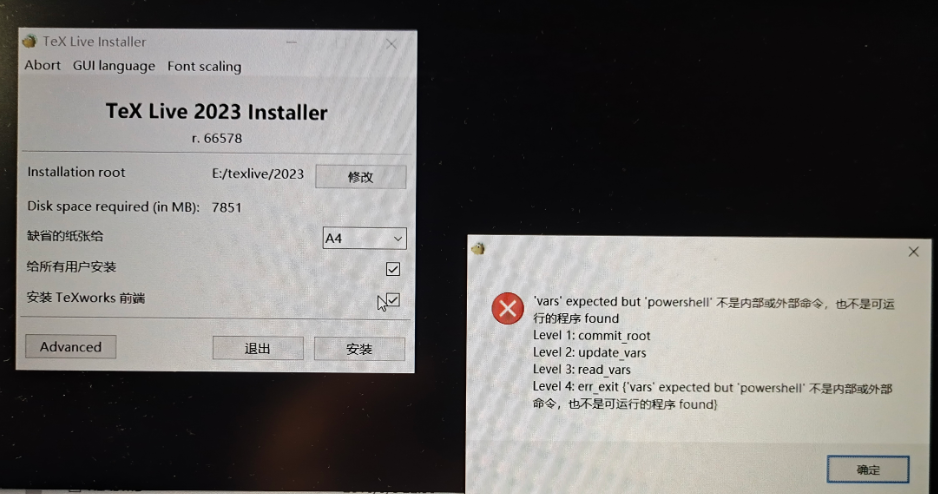
\includegraphics[width=0.8\textwidth]{figure/chap-basic/varexpected.png}
    \caption{Texlive 安装错误}
    \label{fig:varexpected}
\end{figure}

\qaq{解决方法:}参考\href{https://blog.csdn.net/qq_50698753/article/details/130475564}{texlive安装过程中报错 vars expected but powershell},添加如下内容到系统PATH路径中:
\begin{lstlisting}
    %SystemRoot%\System32
    %SystemRoot%
    %SystemRoot%\System32\Wben
    %SystemRoot%\System32\WindowsPowerShell\v1.0
\end{lstlisting}







\section{\LaTeX{} 命令和代码结构}\label{sec:latexstructure}
\subsection{最短的\LaTeX{}代码}\label{subsec:shortlatexcode}

\begin{lstlisting}
\documentclass{article}
\begin{document}
Hello, \LaTeX{}!
\end{document}
\end{lstlisting}

上述代码是\LaTeX{} 排版的最短代码。下面简单介绍\LaTeX{}命令和代码的结构。

\subsection{\LaTeX{}命令和环境}\label{subsec:latexcommands}

\LaTeX{}命令以反斜杠 \hspace{0.2em}\textbackslash\hspace{0.2em} 开头,后面跟一串字母,如\lstinline{\LaTeX}。它们以任意非字母符号为界限。

要注意\LaTeX{} 命令是对大小写敏感的,比如输入 \lstinline{\LaTeX} 命令可以生成错落有致的 \LaTeX{} 字母组合,但输入 \lstinline{\Latex} 或者 \lstinline{\LaTex} 什么都得不到,还会报错;它们与 \lstinline{\LaTeX} 是不同的命令。

一些 \LaTeX{} 命令可以接收一些参数,参数的内容会影响命令的效果。\LaTeX{} 的参数分为可选参数和必选参数。可选参数以方括号 [] 包裹;必选参数一般以花括号 \{\} 包裹。还有些命令可以带一个星号*,带星号和不带星号的命令效果有一定差异,一般是带不带编号,比如章节标题。

\LaTeX{} 中还包括{\bf 环境},用以令一些效果在局部生效,或是生成特殊的文档元素。\LaTeX{} 环境的用法为一对命令 \lstinline{\begin} 和 \lstinline{\end}:
\begin{lstlisting}
\begin{环境名称}[可选参数]{必选参数}
    内容
\end{环境名称}
\end{lstlisting}

有些命令(如 \lstinline{\bfseries})会对其后所有内容产生作用。若要限制其作用范围,则需要使用{\bf 分组}。\LaTeX{} 使用一对花括号
\{\} 作为分组,在分组中使用的命令被限制在分组内,不会影响到分组外的内容。

\subsection{\LaTeX{}源代码结构}\label{subsec:latexsourcestructure}
LATEX 源代码以一个 \lstinline{\documentclass} 命令作为开头,它指定了文档使用的文档类。document 环境当中的内容是文档正文。

在 \lstinline{\documentclass} 和 \lstinline|\begin{document}|之间的位置称为{\bf 导言区}。在导言区中常会使用\lstinline{\usepackage} 命令调用{\bf 宏包},还会进行文档的全局设置。

\begin{lstlisting}

    \documentclass{...} % ...为某文档类,比如artile、book、report等
    % 导言区 
    \usepackage{ctex} %加载 ctex 宏包
    \begin{document}
    这里是正文。
    \end{document}
    %此后内容被忽略。

\end{lstlisting}

在正文区中,一般会包含一些文本、公式、图表、表格等内容。

\section{\LaTeX{} 文档类和宏包}\label{sec:latexclasses}
\subsection{\LaTeX{} 文档类}\label{subsec:latexdocclass}
文档类规定了 \LaTeX{} 源代码所要生成的文档的性质——普通文章、书籍、演示文稿、个人简历等等。\LaTeX{}源代码的开头须用\lstinline{\documentclass} 指定文档类:

\begin{lstlisting}
\documentclass[可选参数]{文档类名称}
\end{lstlisting}

文档类如\LaTeX{}提供的 article、report、book,在其基础上派生的一些文档类,如支持中文排版的 ctexart、ctexrep、ctexbook,或者有其它功能的一些文档类,如 moderncv、beamer 等。\LaTeX{} 提供的基础文档类见表\ref{tab:latex_doc_class},其中前三个习惯上称为“标准文档
类”。

\begin{table}[!h]
    \centering
    \caption{\LaTeX{} 文档类}
    \label{tab:latex_doc_class}
    \begin{tabular}{ll}
        \toprule
        类别      & 说明   \\
        \midrule
        article & 普通文章 \\
        book    & 书籍   \\
        report  & 报告   \\
        \hline
        letter  & 信件   \\
        slides  & 幻灯片  \\
        beamer  & 幻灯片  \\
        memoir  & 书籍类  \\
        acmart  & 科技论文 \\
        \bottomrule
    \end{tabular}
\end{table}

{\bf 可选参数}为文档类指定选项,以全局地规定一些排版的参数,如字号、纸张大小、单双面等等。比如调用 \lstinline{article} 文档类排版文章,指定纸张为 A4 大小,基本字号为 11pt,双面排版:
\begin{lstlisting}
\documentclass[11pt,a4paper,twoside]{article}
\end{lstlisting}

\subsection{\LaTeX{} 宏包}\label{subsec:latexpackage}
在使用 \LaTeX{} 时,时常需要依赖一些扩展来增强或补充\LaTeX{}的功能,比如排版复杂的表格、插入图片、增加颜色甚至超链接等等。这些扩展称为宏包。调用宏包的方法非常类似调用文档类的方法:
\begin{lstlisting}
\usepackage[可选参数]{宏包名称}
\end{lstlisting}
\lstinline{\usepackage} 可以一次性调用多个宏包:

\begin{lstlisting}
    % 一次性调用三个排版表格常用的宏包
    \usepackage{tabularx, makecell, multirow}
\end{lstlisting}

\section{\LaTeX{} 使用到的文件类型}\label{sec:latexfiletypes}

除了源代码文件 \lstinline{.tex} 以外,我们在使用 \LaTeX{} 时还可能接触到各种格式的文件。本节简单介绍一下在使用 \LaTeX{} 时能够经常见到的文件。

每个宏包和文档类都是带特定扩展名的文件,除此之外也有一些文件出现于 \LaTeX{} 模板中:

\begin{itemize}
    \item \lstinline{.sty} 宏包文件。宏包的名称与文件名一致。
    \item \lstinline{.cls} 文档类文件。文档类名称与文件名一致。
    \item \lstinline{.bib} BibTeX 参考文献数据库文件。
    \item \lstinline{.bst} BibTeX 用到的参考文献格式模板。
\end{itemize}

\LaTeX{} 在编译过程中除了生成 .dvi 或 .pdf 格式的文档外,还可能会生成相当多的辅助文件和日志。一些功能如交叉引用、参考文献、目录、索引等,需要先通过编译生成辅助文件,然后再次编译时读入辅助文件得到正确的结果,所以复杂的 \LaTeX{} 源代码可能要编译多次:

\begin{itemize}
    \item \lstinline{.log} 排版引擎生成的日志文件,供排查错误使用。
    \item \lstinline{.aux} \LaTeX{} 生成的主辅助文件,记录交叉引用、目录、参考文献的引用等。
    \item \lstinline{.toc} \LaTeX{} 生成的目录记录文件。
    \item \lstinline{.lof} \LaTeX{} 生成的图片目录记录文件。
    \item \lstinline{.lot} \LaTeX{} 生成的表格目录记录文件。
    \item \lstinline{.bbl} BibTeX 生成的参考文献记录文件。
    \item \lstinline{.blg} BibTeX 生成的日志文件。
    \item \lstinline{.idx} \LaTeX{} 生成的供 makeindex 处理的索引记录文件。
    \item \lstinline{.ind} makeindex 处理 .idx 生成的用于排版的格式化索引文件。
    \item \lstinline{.ilg} makeindex 生成的日志文件。
    \item \lstinline{.out} hyperref 宏包生成的 PDF 书签记录文件。
\end{itemize}

\section{\LaTeX{} 文件组织方式}\label{sec:latexfileorganization}

编写长篇文档时,例如当编写书籍、毕业论文时,单个源文件会使修改、校对变得十分困难。将源文件分割成若干个文件,例如将每章内容单独写在一个文件中,会大大简化修改和校对的工作。

\LaTeX{} 提供了命令 \lstinline{\include} 用来在源代码里插入文件:

\begin{lstlisting}
\include{chapter1}
\include{chapter2}
\include{chapter3}
\end{lstlisting}

需要注意的是,\lstinline{\include} 命令在读入新的文件之前会另起一页。有的时候我们不需要这样,则用\lstinline{\input} 命令,它仅仅只是将文件里面的内容插入到当前位置。

当导言区内容较多时,常常将其单独放置在一个 \lstinline{.tex} 文件中,再用 \lstinline{\input} 命令插入。复杂的图、表、代码等也会用类似的手段处理。

LATEX 还提供了一个 \lstinline{\includeonly} 命令来组织文件,用于导言区,指定只载入某些文件。导言区使用了 \lstinline{\includeonly} 后,正文中不在其列表范围的 \lstinline{\include}命令不会起效:
\begin{lstlisting}
\includeonly{chapter1,chapter3}
\end{lstlisting}


% !TEX root = ../latexnote.tex
\chapter{版面和格式}\label{chap:format}



\section{字体设置}\label{sec:font}

\subsection{字体族}
LaTeX 默认预定义的三种字体族为:罗马字体族,无衬线字体族,打字机字体族。有两种命令可以局部使用这些字体族:
\begin{table}[!h]
  \centering
  \begin{tabular}{ccc}
    \toprule
    字体族 & 带参数命令                  & 声明命令                  \\
    \midrule
    罗马  & \lstinline|\textrm{ }| & \lstinline|\rmfamily| \\
    无衬线 & \lstinline|\textsf{ }| & \lstinline|\sffamily| \\
    打字机 & \lstinline|\texttt{ }| & \lstinline|\ttfamily| \\
    \bottomrule
  \end{tabular}
\end{table}

但是对于中文,没有太多的变体,因此,我们一般使用字体族来区分(宋体,隶书等)。

\begin{explain*}{}
  因此,中文字体的选择与西文字体是分离的,这个要注意。
\end{explain*}
\begin{quote}
  \itshape
  ctex 宏包及其文档类(如ctexart)另外新定义了一些组合字体,可以让中文拥有如同西文一样使用粗体(\lstinline|\bfseries|)和意大利体(\lstinline|\itshape|)的功能,并且重新定义了 \rmfamily 使他同时对中文其作用。 这样就默认了中文的字体组为rm,正常字体是宋体,粗体是黑体,意大利体是楷体,符合我们平时使用的习惯。
\end{quote}
\begin{codeshow}
  我是一个人(宋体),

  \textbf{你呢(黑体)?}

  \textit{不是吧,是汪(楷体)!}
\end{codeshow}

\begin{quote}
  \itshape
  中文的字体族,在ctex宏包及其文档类下进行了一部分预定义,在win下配置了四种字体族,并提供了如下的简化命令来进行使用
\end{quote}
\begin{codeshow}
  {\songti 我是宋体},

  {\heiti 我是黑体},

  {\fangsong 我是仿宋},

  {\kaishu 我是楷体}。
\end{codeshow}


\subsection{使用中文}\label{subsec:chinese}
使用中文需要导入ctex宏包。
\begin{lstlisting}
\usepackage{ctex}
\end{lstlisting}

\subsection{全局字体设置}\label{subsec:global}
\subsubsection{英文字体设置}
设置正文罗马字体族,无衬线字体族和打字机字体族
\begin{lstlisting}
  \setmainfont[可选选项]{字体名}
  \setsansfont[可选选项]{字体名}
  \setmonofont[可选选项]{字体名}
  设置好之后,fontspec会自动找到并匹配相应的粗体,斜体等,令我们使用\bfseries和\itshape也有效,若没有,那需要进行如下的设置。
  \setmainfont[
        BoldFont       = texgyrepagella-bold.otf ,
        ItalicFont     = texgyrepagella-italic.otf ,
        BoldItalicFont = texgyrepagella-bolditalic.otf ]{texgyrepagella-regular.otf}
\end{lstlisting}

\subsubsection{中文字体设置}
\begin{lstlisting}
  \setCJKmainfont[可选选项]{字体名}
  \setCJKsansfont[可选选项]{字体名}
  \setCJKmonofont[可选选项]{字体名}
  \setCJKfamilyfont{中文字体族}{字体名}
\end{lstlisting}

\subsection{局部字体设置}\label{subsec:local}
\subsubsection{英文字体设置}
\begin{lstlisting}
  \usepackage{fontspec}
  \newfontfamily\fugu{Luminari-Regular}
  \newfontfamily\ptmr{PTMono-Regular}
\end{lstlisting}

\subsubsection{中文字体设置}
\begin{lstlisting}
  \newCJKfontfamily\qingsong{FZQKBYSJW--GB1-0}
  或者
  \setCJKfamilyfont{zhsong}{FZShuSong-Z01}
  \newcommand*{\songti}{\CJKfamily{zhsong}}
\end{lstlisting}

可以使用\lstinline|\qingsong|或者\lstinline{\songti}命令来调用宋体字体。

\subsection{文字装饰}\label{subsec:decor}

\LaTeX{} 提供\lstinline{\underline}命令设置下划线。

\begin{codeshow}
  \underline{underlined text}
\end{codeshow}

\lstinline{\underline}命令提供的下划线样式不够灵活,ulem或CJKfntef宏包提供了更灵活的下划线命令,CJKfntef宏包对中文支持更好。

\begin{codeshow}
  \CJKunderdot{important 非常重要}\\
  \CJKunderline{notice 注意}\\
  \CJKunderdblline{urgent 必须}\\
  \CJKunderwave{prompt 提示}\\
  \CJKsout{wrong 错误}\\
  \CJKxout{removed 删除}
\end{codeshow}

\section{分栏}\label{sec:columns}

\LaTeX{} 支持简单的单栏或双栏排版。标准文档类的全局选项 onecolumn、twocolumn 可控制全文分单栏或双栏排版。LATEX 也提供了切换单/双栏排版的命令:

\begin{lstlisting}
\onecolumn
\twocolumn
\end{lstlisting}

切换单/双栏排版时总是会另起一页(\lstinline{\clearpage})。在双栏模式下使用 \lstinline{\newpage} 会换栏而不是换页;\lstinline{\clearpage} 则能够换页。

使用multicol宏包可以实现多栏排版。并且切换不会另起一页。

\begin{lstlisting}
\usepackage{multicol}
\begin{multicols}{2}
  ...
\end{multicols}
\end{lstlisting}

\section{断行、断页、断词}\label{sec:break}

\begin{lstlisting}
\\[length] % \\可以带可选参数length,用于在断行处添加垂直间距,可以在表格公式等地方使用
\newline %不带可选参数,只能用于文本段落中

\newpage %双栏模式下另起一栏,单栏模式下另起一页
\clearpage %单栏、双栏模式下都另起一页
\end{lstlisting}

如果 \LaTeX{} 遇到了很长的英文单词,仅在单词之间的“空格”处断行无法生成疏密程度匀称的段落时,就会考虑从单词中间断开。对于绝大多数单词,\LaTeX{} 能够找到合适的断词位置,在断开的行尾加上连字符\lstinline{-}。如果一些单词没能自动断词,我们可以在单词内手动使用 \lstinline{\-} 命令指定断词的位置:

\begin{codeshow}
  I think this is: su\-per\-cal\-%
  i\-frag\-i\-lis\-tic\-ex\-pi\-%
  al\-i\-do\-ciousu\-per\-cal\-%
  i\-frag\-i\-lis\-tic\.
\end{codeshow}

\section{空格和分段}\label{sec:space}
\LaTeX{} 源代码中,空格键和 Tab 键输入的空白字符视为“空格”。连续的若干个空白字符视为一个空格。一行开头的空格忽略不计。

行末的换行符视为一个空格;但连续两个换行符,也就是空行,会将文字分段。多个空行被视为一个空行。也可以在行末使用 \lstinline{\par} 命令分段。

\begin{codeshow}
  This is a new paragraph. Text text text
  text text   text text text text text text.

  This is a new paragraph.\par
  This is a new paragraph.
\end{codeshow}

\section{注释}\label{sec:comment}
LATEX 用 \% 字符作为注释。在这个字符之后直到行末,所有的字符都被忽略,行末的换行符也不引入空格。

\begin{codeshow}
  This is an % short comment
  % ---
  % Long and organized
  % comments
  % ---
  example: Comments do not bre%
  ak a word.
\end{codeshow}

\section{特殊字符}\label{sec:special}

以下字符在 LATEX 里有特殊用途,如 \% 表示注释,\$、\^{}、\_ 等用于排版数学公式,\& 用于排版表格,等等。直接输入这些字符得不到对应的符号,还往往会出错:

\begin{lstlisting}
  # $ % & { } _ ^ ~ \
\end{lstlisting}

如果想要输入以上符号,需要使用以下带反斜线的形式输入,类似编程语言里的“转义”符号:
\begin{lstlisting}
  \# \$ \% \& \{ \} \_
  \^{} \~{} \textbackslash
\end{lstlisting}

\section{问题}\label{sec:qa}
\subsection{双面空白页}\label{subsec:blankpage}
\qaq{问题:}采用\lstinline{twoside}文档类,使用\lstinline{\cleardoublepage}设置双面空白页,如何去除空白页?

\qaq{解决方法:}在所有\lstinline{\cleardoublepage}之前添加\lstinline{\let\cleardoublepage\clearpage}。
% !TEX root = ../latexnote.tex
\chapter{正文工具}\label{chap:text}
\section{章节}\label{sec:section}

一篇结构化的、条理清晰文档一定是层次分明的,通过不同的命令分割为章、节、小节。三个标准文档类 article、report 和 book\footnote{千万注意是标准文档类,其它文档类,如果不是从标准文档类衍生而来,很可能没有定义或只定义了一部分命令}提供了划分章节的命令:
\begin{lstlisting}
\chapter{章名}
\section{节名}
\subsection{小节名}
\subsubsection{}
\paragraph{}
\subparagraph{}
\end{lstlisting}

带星号版本不进行编号,也不生成目录项和页眉页脚。

\section{目录}\label{sec:toc}

在合适部分添加:
\begin{lstlisting}
\tableofcontents
\end{lstlisting}

上述命令会生成目录,标题默认是“Contents”,可通过下列命令更改:
\begin{lstlisting}
\renewcommand{\contentsname}{目录}
\end{lstlisting}

要正确生成目录项,一般需要编译两次源代码。

如果要将使用\lstinline|\chapter*{}|命令的章节加入目录中,需要使用:
\begin{lstlisting}
\addcontentsline{toc}{level}{title} %level为chapter,section等,title为章节名
\end{lstlisting}

\section{页眉页脚}\label{sec:headerfooter}
\subsection{基本的页眉页脚样式}\label{subsec:basic}

\LaTeX{} 中提供了命令 \lstinline{pagestyle} 来修改页眉页脚的样式:
\begin{lstlisting}
    \pagestyle{page-style}
\end{lstlisting}

命令 \lstinline{thispagestyle} 只影响当页的页眉页脚样式:
\begin{lstlisting}
    \thispagestyle{page-style}
\end{lstlisting}

\lstinline{page-style} 参数为样式的名称,在 \LaTeX{} 里预定义了四类样式,见表 \ref{tbl:pagestyle}。

\begin{table}[htp]
    \centering
    \renewcommand\arraystretch{1.5}
    \caption{\LaTeX{} 预定义的页眉页脚样式}\label{tbl:pagestyle}
    \begin{tabular}{lp{30em}}
        \hline
        {empty}      & 页眉页脚为空                                                              \\
        {plain}      & 页眉为空,页脚为页码。({article} 和 {report} 文档类默认;{book} 文档类的每章第一页也为 plain 格式) \\
        \hline
        {headings}   & 页眉为章节标题和页码,页脚为空。({book} 文档类默认)                                      \\
        {myheadings} & 页眉为页码及 \verb|\markboth| 和 \verb|\markright| 命令手动指定的内容,页脚为空。         \\
        \hline
    \end{tabular}
\end{table}

其中 \texttt{headings} 的情况较为复杂:
\begin{itemize}
    \item {article} 文档类,{twoside} 选项:偶数页为页码和节标题,奇数页为小节标题和页码;
    \item {article} 文档类,{oneside} 选项:页眉为节标题和页码;
    \item {report} 和 {book} 文档类,{twoside} 选项:偶数页为页码和章标题,奇数页为节标题和页码;
    \item {report} 和 {book} 文档类,{oneside} 选项:页眉为章标题和页码。
\end{itemize}

\lstinline{pagenumbering} 命令令我们能够改变页眉页脚中的页码样式:
\begin{lstlisting}
\pagenumbering{style}
\end{lstlisting}

\lstinline{style} 为页码样式,默认为 {arabic}(阿拉伯数字),还可修改为 {roman}(小写罗马数字)、
{Roman}(大写罗马数字)等。注意使用 \lstinline{pagenumbering} 命令后会将页码重置为 1。{book} 文档类的 \lstinline{\frontmatter} 和 \lstinline{\mainmatter} 内部就使用了 \lstinline{\pagenumbering} 命令切换页码样式。

\subsection{手动更改页眉页脚的内容}\label{subsec:marks}

对于 headings 或者 myheadings 样式,\LaTeX{} 允许用户使用命令手动修改页眉上面的内容,
特别是因为使用了 \lstinline{\chapter*} 等命令而无法自动生成页眉页脚的情况:
\begin{lstlisting}
\markright{right-mark}
\markboth{left-mark}{right-mark}
\end{lstlisting}

在双面排版、{headings} 或 {myheadings} 页眉页脚样式下,\lstinline{left-mark} 和 \lstinline{right-mark} 的内容分别预期出现在左页(偶数页)和右页(奇数页)。
事实上 \lstinline{\chapter} 和 \lstinline{\section} 等章节命令内部也使用 \lstinline{\markboth} 或者 \lstinline{\markright} 生成页眉。

\LaTeX{} 默认将页眉的内容都转为大写字母。如果需要保持字母的大小写,可以尝试以下代码\footnote{但是这不能改变页眉的斜体样式(\lstinline{\slshape}),斜体是定义在 {headings} 样式里的。
如果不喜欢斜体,可在 \lstinline{\markboth} 等命令的参数里先使用 \lstinline{\normalfont},再使用想要的字体样式命令,
或直接尝试使用 \lstinline{fancyhdr} 宏包。}:
\begin{lstlisting}
\renewcommand\chaptermark[1]{%
  \markboth{Chapter \thechapter\quad #1}{}}
\renewcommand\sectionmark[1]{%
  \markright{\thesection\quad #1}}
\end{lstlisting}

其中 \lstinline{\thechapter}、\lstinline{\thesection} 等命令为章节计数器的数值。
注意以上代码适用于 {report} 和 {book} 文档类;对于 {article} 文档类,
与两个页眉相关的命令分别为 \lstinline{\sectionmark} 和 \lstinline{\subsectionmark}。

\subsection{{fancyhdr} 宏包}\label{subsec:fancyhdr}

{fancyhdr} 宏包改善了页眉页脚样式的定义方式,允许我们将内容自由安置在页眉和页脚的左、中、右三个位置,还为页眉和页脚各加了一条横线。

{fancyhdr} 自定义了样式名称 {fancy}。使用 {fancyhdr} 宏包定义页眉页脚之前,通常先用 \lstinline|\pagestyle{fancy}| 调用这个样式。
在 {fancyhdr} 中定义页眉页脚的命令为:
\begin{lstlisting}
\fancyhf[position]{...}
\fancyhead[position]{...}
\fancyfoot[position]{...}
\end{lstlisting}
其中 \lstinline{position} 为 L(左)/ C(中)/ R(右)以及与 O(奇数页)/ E(偶数页)字母的组合。\lstinline{\fancyhf} 用于同时定义页眉和页脚,习惯上使用 \lstinline|\fancyhf{}| 来清空页眉页脚的设置。

对于单页文档也可以使用 \lstinline{\lhead} 、 \lstinline{\lfoot} 等命令分别定义页眉和页脚。

\begin{lstlisting}
    \lhead{...}
    \cfoot{...}
    % l、c、r,左 中 右
\end{lstlisting}

下方代码给出了{fancyhdr} 基础用法的一个示例,效果为将章节标题放在和 headings 一致的位置,但使用加粗格式;
页码都放在页脚正中;修改横线宽度,“去掉”页脚的横线。

\begin{lstlisting}
        % 在导言区使用此代码
        \usepackage{fancyhdr}
        \pagestyle{fancy}
        \renewcommand{\chaptermark}[1]{\markboth{#1}{}}
        \renewcommand{\sectionmark}[1]{\markright{\thesection\ #1}}
        \fancyhf{}
        \fancyfoot[C]{\bfseries\thepage}
        \fancyhead[LO]{\bfseries\rightmark}
        \fancyhead[RE]{\bfseries\leftmark}
        \renewcommand{\headrulewidth}{0.4pt} % 注意不用 \setlength
        \renewcommand{\footrulewidth}{0pt}
\end{lstlisting}

{fancyhdr} 还支持用 \lstinline{\fancypagestyle} 为自定义的页眉页脚样式命名,或者重新定义已有的样式如 {plain} 等:
\begin{lstlisting}
% 自定义 myfancy 样式
\fancypagestyle{myfancy}{%
  \fancyhf{}
  \fancyhead{...}
  \fancyfoot{...}
}
% 使用样式
\pagestyle{myfancy}
\end{lstlisting}

\subsection{\lstinline{pifont}宏包触发页脚中文不显示}\label{subsec:pifontconflict}
\qaq{问题:}使用\lstinline{pifont}宏包中的\lstinline{\ding}命令,页脚中文不显示。
\begin{figure}[!h]
    \centering
    \includegraphics[width=\textwidth]{figure/chap-text/pifontconflict.png}
    \caption{页脚中文不显示}
\end{figure}

\qaq{解决方法:}参考\href{https://github.com/CTeX-org/ctex-kit/issues/688}{pifont宏包可能会触发中文不显示},把\lstinline{\makexeCJKactive}加到页眉页脚的开头。
\begin{lstlisting}
    \fancyfoot[C]{  \songti 第\thepage 页  \hspace{0.5em} 共\pageref{LastPage}页}
\end{lstlisting}

\section{脚注}\label{sec:footnote}

脚注命令:
\begin{lstlisting}
\footnote[手动指定序号,可忽略]{脚注内容}
\end{lstlisting}



\section{尾注}\label{sec:endnote}
\LaTeX{} 目前没有提供直接插入尾注的命令,但可以调用endnotes宏包实现。

不常用,暂时略过。

\section{交叉引用}\label{sec:crossref}
可以使用\lstinline|\ref|命令和\lstinline|\label|命令进行交叉引用。在正文中,使用\lstinline|\ref{label}|命令引用,在相应位置使用\lstinline|\label{label}|命令进行标记。

\section{列表}\label{sec:list}

\subsection{无序列表}\label{subsec:itemize}
无序列表环境:

\vspace{2em}
\begin{minipage}{0.45\textwidth}
    \begin{lstlisting}
        \begin{itemize}
            \item 第一项
            \item [-]第二项
            \item [*]第三项
        \end{itemize}
    \end{lstlisting}
\end{minipage}
\begin{minipage}{0.45\textwidth}
    \begin{itemize}
        \item 第一项
        \item [-]第二项
        \item [*]第三项
    \end{itemize}
\end{minipage}

条目之间间距较大,可以使用长度赋值命令将条目环境额外的垂直空白设置为0pt,达到与正文间距一致:

\begin{lstlisting}
    \itemsep=0pt
    \parskip=0pt
\end{lstlisting}


\subsection{有序列表}\label{subsec:enumerate}
有序列表环境:

\vspace{2em}
\begin{minipage}{0.45\textwidth}
    \begin{lstlisting}
        \begin{enumerate}
            \item 第一项
            \item 第二项
            \item 第三项
        \end{enumerate}
    \end{lstlisting}
\end{minipage}
\begin{minipage}{0.45\textwidth}
    \begin{enumerate}
        \item 第一项
        \item 第二项
        \item 第三项
    \end{enumerate}
\end{minipage}

有序列表可以嵌套,可对其序号、标号和前缀进行重定义,但是比较麻烦,可以使用paralist宏包。


\subsection{paralist宏包}\label{subsec:paralist}

暂未接触使用,略过。

\section{代码展示}\label{sec:codeshow}

因为\LaTeX{}排版会自动忽略空白字符等,如果需要按照原格式排版,可以使用\lstinline{verbatim}环境。


\begin{codeshow}
    不使用verbatim环境:
    int main() {
            printf("Hello, world!");
            return 0;
        }

    使用verbatim环境:
    \begin{verbatim}
        int main() {
            printf("Hello, world!");
            return 0;
        }
    \end{verbatim}
\end{codeshow}

行内可以使用\lstinline{\verb|内容|}。

\subsection{lstlisting宏包}\label{subsec:lstlistings}

也可以使用\lstinline{lstlisting}宏包。可以实现复杂的高亮效果,但需要额外的配置。

添加标题:
\begin{verbatim}
\begin{lstlisting}[caption=代码标题]
    代码内容
\end{lstlisting}
\end{verbatim}

设置标题位置,在导言区配置
\begin{lstlisting}
\usepackage{listings}
\lstset{captionpos=b} % 标题位置在下方,t为上方
\end{lstlisting}

可以设置标签:
\begin{lstlisting}
    \renewcommand\lstlistingname{\figurename}
\end{lstlisting}

设置代码环境计数器与图计数器保持一致:
\begin{lstlisting}
\makeatletter
\AtBeginDocument{%
  \let\c@figure\c@lstlisting
  \let\thefigure\thelstlisting
  \let\ftype@lstlisting\ftype@figure % give the floats the same precedence
}
\makeatother
\end{lstlisting}

\section{标点}\label{sec:punctuations}
\subsection{引号}
英文左单引号是\lstinline|`|,右单引号是\lstinline|'|,左双引号是\lstinline|``|,右双引号是\lstinline|''|。

英文下的引号嵌套需要借助\lstinline|\thinspace|命令分隔,比如:

\begin{codeshow}
    ``\thinspace`Max' is here.''

    ```Max' is here.
\end{codeshow}

中文下的单引号和双引号可以用中文输入法直接输入。

\subsection{破折,短横}
英文的短横分为三种:
\begin{itemize}
    \item 连字符:输入一个短横:\lstinline|-|,效果如 daughter-in-law
    \item 数字起止符:输入两个短横:\lstinline|--|,效果如:page 1--2
    \item 破折号:输入三个短横:\lstinline|---|,效果如:Listen—I’m serious.
\end{itemize}

中文的破折号可以直接使用日常的输入方式。

\subsection{下划线与删除线}\label{subsec:decor}

\LaTeX{} 提供\lstinline{\underline}命令设置下划线。

\begin{codeshow}
  \underline{underlined text}
\end{codeshow}

\lstinline{\underline}命令提供的下划线样式不够灵活,ulem或CJKfntef宏包提供了更灵活的下划线命令,CJKfntef宏包对中文支持更好。

\begin{codeshow}
  \CJKunderdot{important 非常重要}\\
  \CJKunderline{notice 注意}\\
  \CJKunderdblline{urgent 必须}\\
  \CJKunderwave{prompt 提示}\\
  \CJKsout{wrong 错误}\\
  \CJKxout{removed 删除}
\end{codeshow}

% !TEX root = ../latexnote.tex
\chapter{图片}\label{chap:figure}
\section{简述}\label{sec:figure-intro}
\LaTeX{} 本身不支持插图功能,需要借助graphicx宏包。

使用 latex + dvipdfmx 编译命令时,调用 graphicx 宏包时要指定 dvipdfmx 选项\footnote{早期常使用 latex + dvips 组合命令,后者将 .dvi 文件转为 .ps 文件(PostScript),可进一步通过 ps2pdf 工具生成 PDF。dvips 和 dvipdfmx 在图形、颜色、超链接等功能的实现上有差别,而 \LaTeX{} 无法识别用户是用 dvips 还是dvipdfmx,所以要指定选项(缺省为 dvips)。};而使用 pdflatex 或 xelatex 命令编译时不需要。

下表给出了不同编译命令支持的图片格式:

\begin{table}[htp]
    \centering
    \caption{各种编译方式支持的主流图片格式}\label{tbl:figure-format}
    \begin{tabular}{*{3}{l}}
        \hline
        \textbf{格式}              & \textbf{矢量图} & \textbf{位图}      \\
        \hline
        {latex + dvipdfmx}       & {.eps}       & N/A              \\
        \quad (调用 {bmpsize} 宏包 ) & {.eps .pdf}  & {.jpg .png .bmp} \\[.3\baselineskip]
        {pdflatex}               & {.pdf}       & {.jpg .png}      \\
        \quad (调用 {epstopdf} 宏包) & {.pdf .eps}  & {.jpg .png}      \\[.3\baselineskip]
        {xelatex}                & {.pdf .eps}  & {.jpg .png .bmp} \\
        \hline
    \end{tabular}
    \begin{quote}\footnotesize
        注:在较新的 \TeX{} 发行版中,{latex + dvipdfmx} 和 {pdf\-latex} 命令可不依赖宏包,支持原来需要宏包扩展的图片格式
        (但 {pdf\-latex} 命令仍不支持 {.bmp} 格式的位图)。
    \end{quote}
\end{table}

引入graphicx 宏包后,可使用 \lstinline|\includegraphics| 命令插入图片,其语法为:


\begin{lstlisting}
\includegraphics[options]{file} % options可指定图片属性,如width=
\end{lstlisting}


其中,options 可选参数有:

\begin{table}[htp]
    \centering
    \caption{ \lstinline{\includegraphics} 命令的可选参数}\label{tbl:graphics-options}
    \begin{tabular}{lp{18em}}
        \hline
        \textbf{参数}     & \textbf{含义}          \\
        \hline
        width={width}   & 将图片缩放到宽度为{width}     \\
        height={height} & 将图片缩放到高度为{height}    \\
        scale={scale}   & 将图片相对于原尺寸缩放{scale} 倍 \\
        angle={angle}   & 将图片逆时针旋转{angle} 度    \\
        \hline
    \end{tabular}
\end{table}

\section{浮动体}\label{sec:figure-float}

浮动体将图、表与其标题定义为整体,然后动态排版,以解决图、表卡在换页处造成的过长的垂直空白的问题。图片的浮动体是figure。

下面是一个例子:
\begin{lstlisting}
\begin{figure}[htbp]
    \centering
    \includegraphics[width=0.8\textwidth]{example-image}
    \caption{This is an example image.}
    \label{fig:example-image}
\end{figure}
\end{lstlisting}

参数htbp表示浮动体的位置,h表示插入此处、t表示在页面上端,b表示在页面下端、p表示允许浮动体单开一页。

\section{问题}
\subsection{\lstinline{subcaption}修改标题}\label{subsec:figure-subcaption}
\qaq{问题:}加载\lstinline|subcaption|宏包后,会修改caption设置的标题格式。

\qaq{解决方法:}参考\href{https://tex.stackexchange.com/questions/154435/ieee-template-and-caption-false-option-for-subcaption-package}{IEEE template and \lstinline{caption=false} option for subcaption package?}
\begin{lstlisting}
\makeatletter
\let\MYcaption\@makecaption
\makeatother

\usepackage{subcaption}

\makeatletter
\let\@makecaption\MYcaption
\makeatother
\end{lstlisting}

\subsection{\lstinline{IEEE Access}模板与tikz宏包冲突}\label{subsec:figure-ieeeaccess}
\qaq{问题:}使用\lstinline{IEEE Access}模板时,如果导入\lstinline{tikz}宏包会导致编译失败。

\qaq{解决方法:}参考\href{https://www.cnblogs.com/greatestchen/p/17006317.html}{解决Overleaf 中 IEEE Access 模板与 Tikz 包的冲突}

在 \lstinline|ieeeaccess.cls| 文件 中,将 \lstinline|\def\year| 改成 \lstinline|\def\Year|

在 \lstinline|access.tex| 文件 中,将下列语句加在 \lstinline|\usepackage{tikz}| 后面:
\begin{lstlisting}
    \NewSpotColorSpace{PANTONE}
    \AddSpotColor{PANTONE} {PANTONE3015C} {PANTONE\SpotSpace 3015\SpotSpace C} {1 0.3 0 0.2}
    \SetPageColorSpace{PANTONE}
\end{lstlisting}  
% !TEX root = ../latexnote.tex
\chapter{表格}\label{chap:table}

\section{基本表格}\label{sec:basic-table}

表格和图片类似,也有一个浮动体环境为table。

表格最基本的环境为tabular,用法如下:
\begin{lstlisting}
\begin{tabular}[可选参数]{|c|c|c|}
\hline
第一列 & 第二列 & 第三列 \\
\hline
1 & 2 & 3 \\
4 & 5 & 6 \\
\hline
\end{tabular}
\end{lstlisting}

其中\lstinline{|c|c|c|}是列格式标记,详细见\ref{sec:liegeshi},c表示列居中,|表示列之间有竖线。使用\&用来分割列,使用\lstinline|\\|表示换行。\lstinline{\hline}用来绘制行之间的横线。

\subsection{修改表格线}\label{sec:modify-table-line}
可在tabular环境外修改全部表格线的粗细,如\lstinline|\setlength{\arrayrulewidth}{2pt}|或\lstinline{\arrayrulewidth=2pt}。

如果需要单独修改表格线,可采用如下方法:

1)修改垂直表格线,使用array宏包提供的新列格式选项定义命令:
\begin{lstlisting}
\newcolumntype{新选项名称}[参数数量]{列格式}
\newcolumntype{I}{!{\vrule width 2pt}}
\end{lstlisting}
\begin{codeshow}
    \centering
    \newcolumntype{I}{!{\vrule width 2pt}}
    \begin{tabular}{|cIcIc|}
        \hline
        \multicolumn{3}{IcI}{垂直线粗细更改} \\
        \hline
        7 & 5 & 3                     \\
        \hline
        6 & 1 & 8                     \\
        \hline
    \end{tabular}
\end{codeshow}

2)修改水平表格线,可使用booktabs宏包,该宏包可以任意修改水平线粗细,还可以在上下附加一段垂直空白。

\begin{codeshow}
    \centering
    \begin{tabular}{|c|c|c|}
        \hline
        \multicolumn{3}{|c|}{水平表格线粗细更改} \\
        \specialrule{2pt}{0pt}{0pt}
        7 & 5 & 3                       \\
        \hline
        6 & 1 & 8                       \\
        \hline
    \end{tabular}
\end{codeshow}

\subsection{列格式}\label{sec:column-format}
\label{sec:liegeshi}

基本列格式如下表所示:

\begin{table}[htp]
    \centering
    \caption{\LaTeX{} 表格列格式}\label{tbl:table-column-spec}
    \begin{tabular}{*{2}{l}}
        \hline
        \textbf{列格式} & \textbf{说明}            \\
        \hline
        l/c/r        & 单元格内容左对齐/居中/右对齐,不折行    \\
        p\{width\}   & 单元格宽度固定为 {width},可自动折行 \\
        |            & 绘制竖线                   \\
        @\{string\}  & 自定义内容 {string}         \\
        \hline
    \end{tabular}
\end{table}

格中每行的单元格数目不能多于列格式里 l/c/r/p 的总数(可以少于这个总数),否则出错。

@ 格式可在单元格前后插入任意的文本,但同时它也消除了单元格前后额外添加的间距。@格式可以适当使用以充当“竖线”。特别地,\lstinline|@{}| 可直接用来消除单元格前后的间距。

另外\LaTeX{} 还提供了简便的将格式参数重复的写法 \lstinline|*{⟨n⟩}{⟨column-spec⟩}|,比如以下两种写法是等效的:
\begin{lstlisting}
    \begin{tabular}{|c|c|c|c|c|p{4em}|p{4em}|}
    \begin{tabular}{|*{5}{c|}*{2}{p{4em}|}}
\end{lstlisting}


\subsection{列宽}\label{sec:column-width}

\LaTeX{} 本身提供了 tabular* 环境用来排版定宽表格,但是不太方便使用,比如要用到 @ 格式插入额外命令,令单元格之间的间距为 \lstinline{\fill},但即使这样仍然有瑕疵:

\begin{codeshow}
    \begin{tabular*}{14em}%
        {@{\extracolsep{\fill}}|c|c|c|c|}
        \hline
        A & B & C & D \\ \hline
        a & b & c & d \\ \hline
    \end{tabular*}
\end{codeshow}

tabularx 宏包为我们提供了方便的解决方案。它引入了一个 X 列格式,类似 p 列格式,不过会根据表格宽度自动计算列宽,多个 X 列格式平均分配列宽。X 列格式也可以用 array 里的辅助格式修饰对齐方式:

\begin{codeshow}
    % \usepackage{array,tabularx}
    \begin{tabularx}{14em}%
        {|*{4}{>{\centering\arraybackslash}X|}}
        \hline
        A & B & C & D \\ \hline
        a & b & c & d \\ \hline
    \end{tabularx}
\end{codeshow}

\subsection{行距}\label{sec:row-spacing}

修改参数 \lstinline{\arraystretch} 可以得到行距更加宽松的表格:
\begin{lstlisting}
    \renewcommand\arraystretch{1.8}
\end{lstlisting}

另一种增加间距的办法是给换行命令 \lstinline|\\| 添加可选参数,在这一行下面加额外的间距,适合用于在行间不加横线的表格:


\subsection{表格标题}\label{sec:table-title}

表格标题可以用\lstinline{\caption}命令设置,默认只能在浮动体环境内部使用。

也可以在导言区添加如下命令,在浮动体外使用\lstinline{\figcaption}和\lstinline{\tabcaption}为图表添加标题。为了防止标题和图表不在一页,可以使用minipage环境将它们包起来。

\begin{lstlisting}
    \makeatletter
    \newcommand\figcaption{def\@captype{figure}\caption}
    \newcommand\tabcaption{def\@captype{table}\caption}
    \makeatother
\end{lstlisting}



\section{复杂表格}\label{sec:complex-table}

\subsection{合并单元格}\label{sec:merge-cell}

1)跨列

使用\lstinline{\multicolumn}命令可以合并列:
\begin{lstlisting}
    \multicolumn{合并列数目}{列格式}{内容}
\end{lstlisting}

2)跨行

跨行需要引入multirow宏包,使用\lstinline{\multirow}命令:
\begin{lstlisting}
    \multirow{合并行数目}{宽度}{内容} %宽度可以填*以使用自然宽度
\end{lstlisting}

既跨行又跨列时,需要把\lstinline{\multirow}命令放在\lstinline{\multicolumn}命令内部。

\begin{codeshow}
    \centering
    \begin{center}
        \begin{tabular}{|c|c|c|}
            \hline
            \multirow{2}{2cm}{A Text!}
                                     & ABC & DEF \\
            \cline{2-3}              & abc & def \\
            \hline
            \multicolumn{2}{|c|}
            {\multirow{2}*{Nothing}} & XYZ       \\
            \multicolumn{2}{|c|}{}   & xyz       \\
            \hline
        \end{tabular}
    \end{center}
\end{codeshow}

\subsection{单元格旋转}\label{sec:cell-rotate}
使用\lstinline{\rotatebox}命令可以旋转单元格内容。

\begin{codeshow}
    \begin{tabular}{|c|c|c|}
        \hline
        \rotatebox{90}{A}           & B                 & C \\
        \hline
        D                           & \rotatebox{45}{E} & F \\
        \hline
        \rotatebox[origin=l]{90}{G} & H                 & I \\
        \hline
    \end{tabular}
\end{codeshow}




\section{问题}

\subsection{longtable与arydshln宏包冲突}\label{subsec:longtable-arydshln-conflict}
\qaq{问题:}最近帮人debug,使用longtable排版报错。
\begin{figure}[!h]
    \centering
    \includegraphics[width=0.4\textwidth]{figure/chap-tab/ary1.png}
    \caption{报错信息}
\end{figure}

\qaq{解决方法:}参考\href{https://zhuanlan.zhihu.com/p/667681242}{LaTeX:arydshln与longtable的冲突及教训 - 知乎 (zhihu.com)}, 发现longtable与arydshln宏包存在冲突,arydshln宏包重定义了\lstinline{\hline},可以采用如下解决方法:
\begin{enumerate}
    \item 注释掉\lstinline|\usepackage{arydshln}|。
    \item 将\lstinline|\usepackage{arydshln}|放于\lstinline|\usepackage{longtable}|之后
\end{enumerate}

\subsection{cline命令 undefined control sequence报错}\label{subsec:cline-undefined-control-sequence-error}
\qaq{问题:}使用Springer模板制作表格,使用\lstinline{\cline}命令报错,提示\lstinline{undefined control sequence}。

\qaq{解决方法:}Springer模板重新定义了\lstinline{\cline}命令,找到Springer模板的\lstinline{sn-jnl.cls}文件,将下面一行注释掉:
\begin{lstlisting}
    \let\cline\cmidrule
\end{lstlisting}

\subsection{multirow宏包居中}\label{subsec:multirow-center}

\qaq{问题:}列格式设置为居中,但是使用multirow多行合并内容不会居中

\qaq{解决方法:}添加如下命令:
\begin{lstlisting}
\renewcommand{\multirowsetup}{\centering}
\end{lstlisting}

\subsection{\lstinline|cline|命令在\lstinline|colortbl|宏包中被遮盖}\label{subsec:cline-colortbl-error}
\qaq{问题:}使用\lstinline{colortbl}宏包,\lstinline{\cline}命令在表格中被遮盖,导致表格线不显示。如图\ref{fig:cline-colortbl-error}所示。

\begin{figure}[!h]
    \centering
    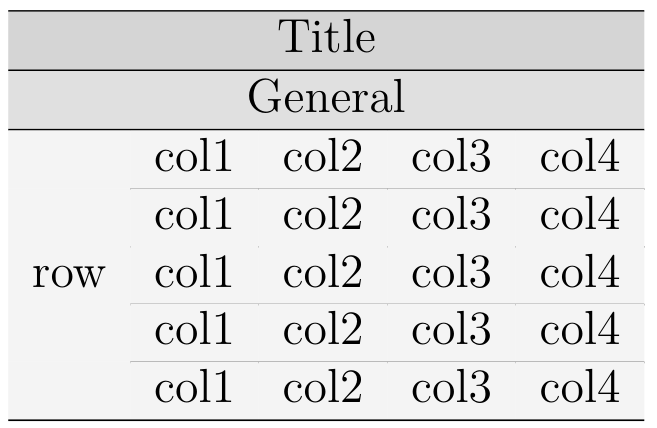
\includegraphics[width=0.4\textwidth]{figure/chap-tab/cline-colortbl-error.png}
    \caption{{cline}命令在{colortbl}宏包中被遮盖}
    \label{fig:cline-colortbl-error}
\end{figure}

MWE如下:
\begin{lstlisting}
\documentclass[a4paper,12pt]{article}

\usepackage{multirow}
\usepackage{array}
\usepackage[table]{xcolor}  % 用于淡灰色背景
\usepackage{hhline}

\begin{document}

\begin{tabular}{ccccc}
    \hline
    \rowcolor{gray!40}\multicolumn{5}{c}{Title}                         \\
    \hline
    \rowcolor{gray!30}\multicolumn{5}{c}{General}                       \\
    \hline
    \rowcolor{gray!10}                      & col1 & col2 & col3 & col4 \\
    \cline{2-5}
    \rowcolor{gray!10}                      & col1 & col2 & col3 & col4 \\
    \cline{2-5}
    \rowcolor{gray!10}                      & col1 & col2 & col3 & col4 \\
    \cline{2-5}
    \rowcolor{gray!10}                      & col1 & col2 & col3 & col4 \\
    \cline{2-5}
    \rowcolor{gray!10}\multirow{-5}{*}{row} & col1 & col2 & col3 & col4 \\
    \hline
\end{tabular}

\end{document}
\end{lstlisting}

\qaq{解决方法:}使用\lstinline|hhline|宏包中的\lstinline|\hhline|命令代替\lstinline|\cline|命令,如图\ref{fig:cline-colortbl-sol}所示。
\begin{lstlisting}
    \documentclass[a4paper,12pt]{article}

\usepackage{multirow}
\usepackage{array}
\usepackage[table]{xcolor}  % 用于淡灰色背景
\usepackage{hhline}

\begin{document}

\begin{tabular}{ccccc}
    \hline
    \rowcolor{gray!40}\multicolumn{5}{c}{Title}                         \\
    \hline
    \rowcolor{gray!30}\multicolumn{5}{c}{General}                       \\
    \hline
    \rowcolor{gray!10}                      & col1 & col2 & col3 & col4 \\
    \hhline{*1{>{\arrayrulecolor{gray!10}}-}>{\arrayrulecolor{black}}|*4{-}|}
    \rowcolor{gray!10}                      & col1 & col2 & col3 & col4 \\
    \hhline{*1{>{\arrayrulecolor{gray!10}}-}>{\arrayrulecolor{black}}|*4{-}|}
    \rowcolor{gray!10}                      & col1 & col2 & col3 & col4 \\
    \hhline{*1{>{\arrayrulecolor{gray!10}}-}>{\arrayrulecolor{black}}|*4{-}|}
    \rowcolor{gray!10}                      & col1 & col2 & col3 & col4 \\
    \hhline{*1{>{\arrayrulecolor{gray!10}}-}>{\arrayrulecolor{black}}|*4{-}|}
    \rowcolor{gray!10}\multirow{-5}{*}{row} & col1 & col2 & col3 & col4 \\
    \hline
\end{tabular}

\end{document}
\end{lstlisting}

\begin{figure}[!h]
    \centering
    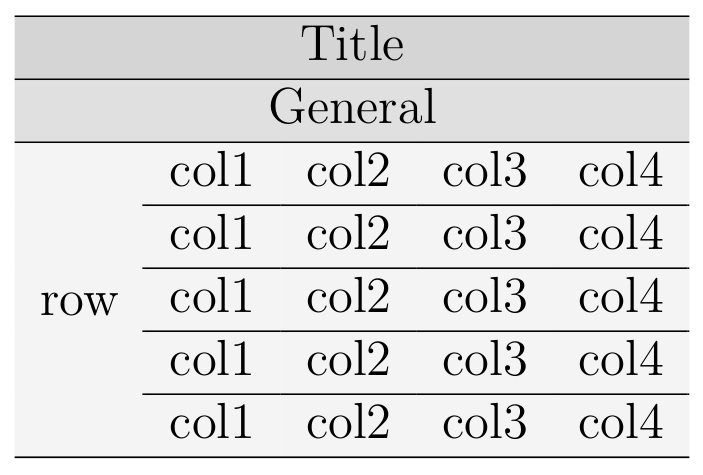
\includegraphics[width=0.4\textwidth]{figure/chap-tab/cline-colortbl-sol.png}
    \caption{{hhline}命令在{colortbl}宏包中正常显示}
    \label{fig:cline-colortbl-sol}
\end{figure}

\subsection{\lstinline|tabularx|表格垂直居中}\label{subsec:tabularx-center}

\qaq{问题:}使用\lstinline{tabularx}宏包,表格内容顶部居中

\begin{codeshow}
    \begin{tabularx}{0.3\textwidth}{|X|X|}
        \hline
        text & this is a long text long 
        text long text long text long text\\
        \hline
    \end{tabularx}
\end{codeshow}


\qaq{解决方法:}添加命令\lstinline|\def\tabularxcolumn#1{m{#1}}|,需要导入\lstinline{array}宏包。

\begin{codeshow}
    \def\tabularxcolumn#1{m{#1}}
    \begin{tabularx}{0.3\textwidth}{|X|X|}
        \hline
        text & this is a long text long 
        text long text long text long text\\
        \hline
    \end{tabularx}
\end{codeshow}
% !TEX root = ../latexnote.tex
% Definitions
\def\lsym{$\mathsurround=0pt {}^\ell$}
\def\LSYM    #1{$#1$     & \texttt{\string#1}\lsym}

\def\SYM     #1{$#1$     & \texttt{\string#1}}
\def\BIGSYM  #1{$#1$     & $\displaystyle #1$ & \texttt{\string#1}}
\def\ACC   #1#2{$#1{#2}$ & \texttt{\string#1}\{#2\}}
\def\DEL     #1{$\big#1 \bigg#1$ & \texttt{\string#1}}

\def\AMSSYM  #1{$#1$     & \texttt{\string#1}}
% These symbols rely on `amsmath' package
\def\AMSM    #1{$#1$     & \textcolor{blue}{\texttt{\string#1}}}
\def\AMSACC#1#2{$#1{#2}$ & \textcolor{blue}{\texttt{\string#1}}\{#2\}}
\def\AMSBIG  #1{$#1$     & $\displaystyle #1$ & \textcolor{blue}{\texttt{\string#1}}}

\def\SC      #1{#1       & \texttt{\string#1}}

\newenvironment{symbols}[1]%
{\small\def\arraystretch{1.1}
    \begin{tabular}{@{}#1@{}}}%
        {\end{tabular}}

\DeclareRobustCommand*\amscmd[1]{\textcolor{blue}{\lstinline{#1}}}
\DeclareRobustCommand*\amsenv[1]{\textcolor{blue}{\lstinline{#1}}}

\chapter{数学公式}\label{chap:math}
\section{行内公式}\label{sec:inline}
行内公式使用\lstinline|\$|和\lstinline|\$|包裹,如:

\begin{codeshow}
    行内公式测试$a=b$
\end{codeshow}

\section{行间公式}\label{sec:display}
行间公式使用\lstinline|\begin{equation}|和\lstinline|\end{equation}|包裹,如:

\begin{codeshow}
    \begin{equation}
        a+b=c
    \end{equation}
\end{codeshow}

\lstinline{equation} 环境为公式自动生成一个编号,这个编号可以用 \lstinline{label} 和 \lstinline{ref} 生成交叉引用,
\lstinline{amsmath} 的 \amscmd{eqref} 命令甚至为引用自动加上圆括号;还可以用 \amscmd{tag} 命令手动修改公式的编号,
或者用 \amscmd{notag} 命令取消为公式编号(与之基本等效的命令是 \lstinline{nonumber})。

\begin{codeshow}
    The Pythagorean theorem is:
    \begin{equation}
        a^2 + b^2 = c^2 \label{pythagorean}
    \end{equation}
    Equation \eqref{pythagorean} is
    called `Gougu theorem' in Chinese.

    It's wrong to say
    \begin{equation}
        1 + 1 = 3 \tag{dumb}
    \end{equation}
    or
    \begin{equation}
        1 + 1 = 4 \notag
    \end{equation}
\end{codeshow}


使用\lstinline|\begin{equation*}|和\lstinline|\end{equation*}|包裹的公式不带编号,如:

\begin{codeshow}
    \begin{equation*}
        a+b=c
    \end{equation*}
\end{codeshow}

\section{数学符号}\label{sec:math-symbols}
\subsection{指数、上下标和导数}\label{subsec:math-scripts}
在 \LaTeX{} 中用 \texttt\textasciicircum 和 \texttt\textunderscore 标明上下标。
注意上下标的内容(子公式)一般需要\textbf{用花括号包裹},否则上下标只对后面的一个符号起作用。

\begin{codeshow}
    $p^3_{ij} \qquad
        m_\mathrm{Knuth}\qquad
        \sum_{k=1}^3 k $\\[5pt]
    $a^x+y \neq a^{x+y}\qquad
        e^{x^2} \neq {e^x}^2$
\end{codeshow}

{导数符号\texttt' ($a'$)}
导数符号\texttt'(${}'$)是一类特殊的上标,可连续使用,但只能在\textbf{其后}添加其他上标:

\begin{codeshow}
    $f(x) = x^2 \quad f'(x)
        = 2x \quad f''^{2}(x) = 4$
\end{codeshow}

\subsection{分式和根式}\label{subsec:frac-sqrt}
分式使用 \lstinline|\frac{分子}{分母}| 来书写。分式的大小在行间公式中是正常大小,而在行内被极度压缩。
\lstinline{amsmath} 提供了方便的命令 \amscmd{dfrac} 和 \amscmd{tfrac},令用户能够在行内使用正常大小的分式,或是反过来。

\begin{codeshow}
    In display style:
    \[
        3/8 \qquad \frac{3}{8}
        \qquad \tfrac{3}{8}
    \]
    In text style:
    $1\frac{1}{2}$~hours \qquad
    $1\dfrac{1}{2}$~hours
\end{codeshow}

一般的根式使用 \lstinline|\sqrt{ }|;表示 $n$ 次方根时写成 \lstinline|\sqrt[n]{ }|。

\begin{codeshow}
    $\sqrt{x} \Leftrightarrow x^{1/2}
        \quad \sqrt[3]{2}
        \quad \sqrt{x^{2} + \sqrt{y}}$
\end{codeshow}


特殊的分式形式,如二项式结构,由 \lstinline{amsmath} 宏包的 \amscmd{binom} 命令生成:

\begin{codeshow}
    Pascal's rule is
    \[
        \binom{n}{k} =\binom{n-1}{k}
        + \binom{n-1}{k-1}
    \]
\end{codeshow}

\section{符号表}\label{sec:math-tables}

有几个注意事项:
\begin{enumerate}
    \item 本节选自\href{https://github.com/CTeX-org/lshort-zh-cn/tree/master}{The Not So Short Introduction To LaTeX2ε (Chinese Edition)}
    \item \textcolor{blue}{蓝色}的命令依赖 \lstinline{amsmath} 宏包(非 \lstinline{amssymb} 宏包);
    \item 带有角标\lsym 的符号命令依赖 \lstinline{latexsym} 宏包。
\end{enumerate}

\subsection{\LaTeX{} 普通符号}
\subsubsection{文本/数学模式通用符号}
\begin{table}[htp]
    \centering
    \caption{文本/数学模式通用符号}\label{tbl:general-syms}
    \begin{quote}\footnotesize%
        这些符号可用于文本和数学模式。
    \end{quote}
    \begin{symbols}{*4{cl}}
        \hline
        \SC{\{}    &  \SC{\}}  &  \SC{\$}         &  \SC{\%}               \\
        \SC{\dag}  &  \SC{\S}  &  \SC{\copyright} &  \SC{\dots}            \\
        \SC{\ddag} &  \SC{\P}  &  \SC{\pounds}    &                        \\
        \hline
    \end{symbols}
\end{table}

\subsubsection{希腊字母}
\begin{table}[H]
    \centering
    \caption{希腊字母} \label{tbl:math-greek}
    \begin{quote}\footnotesize%
        % \cmd{Alpha},\cmd{Beta} 等希腊字母符号不存在,因为它们和拉丁字母 A,B 等一模一样;
        % 小写字母里也不存在 \cmd{omicron},直接用拉丁字母 $o$ 代替。
    \end{quote}
    \begin{symbols}{*4{cl}}
        \hline
        \SYM{\alpha}     & \SYM{\theta}     & \SYM{o}          & \SYM{\upsilon}  \\
        \SYM{\beta}      & \SYM{\vartheta}  & \SYM{\pi}        & \SYM{\phi}      \\
        \SYM{\gamma}     & \SYM{\iota}      & \SYM{\varpi}     & \SYM{\varphi}   \\
        \SYM{\delta}     & \SYM{\kappa}     & \SYM{\rho}       & \SYM{\chi}      \\
        \SYM{\epsilon}   & \SYM{\lambda}    & \SYM{\varrho}    & \SYM{\psi}      \\
        \SYM{\varepsilon}& \SYM{\mu}        & \SYM{\sigma}     & \SYM{\omega}    \\
        \SYM{\zeta}      & \SYM{\nu}        & \SYM{\varsigma}  &                 \\
        \SYM{\eta}       & \SYM{\xi}        & \SYM{\tau}       &                 \\[1ex]
        \SYM{\Gamma}     & \SYM{\Lambda}    & \SYM{\Sigma}     & \SYM{\Psi}      \\
        \SYM{\Delta}     & \SYM{\Xi}        & \SYM{\Upsilon}   & \SYM{\Omega}    \\
        \SYM{\Theta}     & \SYM{\Pi}        & \SYM{\Phi}       &                 \\[1ex]
        \AMSM{\varGamma} & \AMSM{\varLambda}& \AMSM{\varSigma}  & \AMSM{\varPsi}      \\
        \AMSM{\varDelta} & \AMSM{\varXi}    & \AMSM{\varUpsilon}& \AMSM{\varOmega}    \\
        \AMSM{\varTheta} & \AMSM{\varPi}    & \AMSM{\varPhi}    &                 \\
        \hline
    \end{symbols}
\end{table}


\subsubsection{二元关系符}
\begin{table}[H]
    \centering
    \caption{二元关系符} \label{tbl:math-rel}
    \begin{quote}\footnotesize%
        所有的二元关系符都可以加 \lstinline{not} 前缀得到相反意义的关系符,例如 \lstinline{not}\texttt{=} 就得到不等号(同 \lstinline{ne})。
    \end{quote}
    \begin{symbols}{*3{cl}}
        \hline
        \SYM{<}              & \SYM{>}                    & \SYM{=}          \\
        \SYM{\leq} or \verb|\le|   & \SYM{\geq} or \verb|\ge| & \SYM{\equiv}     \\
        \SYM{\ll}            & \SYM{\gg}                  & \SYM{\doteq}     \\
        \SYM{\prec}          & \SYM{\succ}                & \SYM{\sim}       \\
        \SYM{\preceq}        & \SYM{\succeq}              & \SYM{\simeq}     \\
        \SYM{\subset}        & \SYM{\supset}              & \SYM{\approx}    \\
        \SYM{\subseteq}      & \SYM{\supseteq}            & \SYM{\cong}      \\
        \LSYM{\sqsubset}     & \LSYM{\sqsupset}           & \LSYM{\Join}     \\
        \SYM{\sqsubseteq}    & \SYM{\sqsupseteq}          & \SYM{\bowtie}    \\
        \SYM{\in}            & \SYM{\ni}, \verb|\owns|      & \SYM{\propto}    \\
        \SYM{\vdash}         & \SYM{\dashv}               & \SYM{\models}    \\
        \SYM{\mid}           & \SYM{\parallel}            & \SYM{\perp}      \\
        \SYM{\smile}         & \SYM{\frown}               & \SYM{\asymp}     \\
        \SYM{:}              & \SYM{\notin}               & \SYM{\neq} or \verb|\ne| \\
        \hline
    \end{symbols}
\end{table}

\subsubsection{二元运算符}
\begin{table}[H]
    \centering
    \caption{二元运算符}\label{tbl:math-op}
    \begin{symbols}{*3{cl}}
        \hline
        \SYM{+}              & \SYM{-}              &                     \\
        \SYM{\pm}            & \SYM{\mp}            & \SYM{\triangleleft} \\
        \SYM{\cdot}          & \SYM{\div}           & \SYM{\triangleright}\\
        \SYM{\times}         & \SYM{\setminus}      & \SYM{\star}         \\
        \SYM{\cup}           & \SYM{\cap}           & \SYM{\ast}          \\
        \SYM{\sqcup}         & \SYM{\sqcap}         & \SYM{\circ}         \\
        \SYM{\vee}, \verb|\lor| & \SYM{\wedge},\verb|\land|  & \SYM{\bullet}   \\
        \SYM{\oplus}         & \SYM{\ominus}        & \SYM{\diamond}      \\
        \SYM{\odot}          & \SYM{\oslash}        & \SYM{\uplus}        \\
        \SYM{\otimes}        & \SYM{\bigcirc}       & \SYM{\amalg}        \\
        \SYM{\bigtriangleup} &\SYM{\bigtriangledown}& \SYM{\dagger}       \\
        \LSYM{\lhd}          & \LSYM{\rhd}          & \SYM{\ddagger}      \\
        \LSYM{\unlhd}        & \LSYM{\unrhd}        & \SYM{\wr}           \\
        \hline
    \end{symbols}
\end{table}

\subsubsection{巨算符}
\begin{table}[H]
    \centering
    \caption{巨算符}\label{tbl:math-bigop}
    \def\arraystretch{2.5}
    \begin{symbols}{*3{ccl}}
        \hline
        \BIGSYM{\sum}      & \BIGSYM{\bigcup}   & \BIGSYM{\bigvee}  \\
        \BIGSYM{\prod}     & \BIGSYM{\bigcap}   & \BIGSYM{\bigwedge} \\
        \BIGSYM{\coprod}   & \BIGSYM{\bigsqcup} & \BIGSYM{\biguplus} \\
        \BIGSYM{\int}      & \BIGSYM{\oint}     & \BIGSYM{\bigodot} \\
        \BIGSYM{\bigoplus} & \BIGSYM{\bigotimes} & \\
        \AMSBIG{\iint}     & \AMSBIG{\iiint}    & \AMSBIG{\iiiint}  \\
        \AMSBIG{\idotsint} &                    & \\
        \hline
    \end{symbols}
\end{table}

\subsubsection{数学重音符号}
\begin{table}[H]
    \centering
    \caption{数学重音符号}\label{tbl:math-accents}
    \begin{quote}\footnotesize%
        最后一个 \lstinline{\wideparen} 依赖 \lstinline{yhmath} 宏包。
    \end{quote}
    \begin{symbols}{*3{cl}}
        \hline
        \ACC{\hat}{a}   & \ACC{\check}{a} & \ACC{\tilde}{a}       \\
        \ACC{\acute}{a} & \ACC{\grave}{a} & \ACC{\breve}{a}       \\
        \ACC{\bar}{a}   & \ACC{\vec}{a}   & \ACC{\mathring}{a}    \\
        \ACC{\dot}{a}   & \ACC{\ddot}{a}  & \AMSACC{\dddot}{a}    \\
        \AMSACC{\ddddot}{a} \\[1ex]
        \ACC{\widehat}{AAA} & \ACC{\widetilde}{AAA} & \ACC{\wideparen}{AAA} \\
        \hline
    \end{symbols}
\end{table}

\subsubsection{箭头}
\begin{table}[H]
    \centering
    \caption{箭头} \label{tbl:math-arrows}
    \begin{symbols}{*2{cl}}
        \hline
        \SYM{\leftarrow} or \verb|\gets| & \SYM{\longleftarrow} \\
        \SYM{\rightarrow} or \verb|\to|   & \SYM{\longrightarrow} \\
        \SYM{\leftrightarrow}    & \SYM{\longleftrightarrow} \\
        \SYM{\Leftarrow}         & \SYM{\Longleftarrow}     \\
        \SYM{\Rightarrow}        & \SYM{\Longrightarrow}    \\
        \SYM{\Leftrightarrow}    & \SYM{\Longleftrightarrow}\\
        \SYM{\mapsto}            & \SYM{\longmapsto}        \\
        \SYM{\hookleftarrow}     & \SYM{\hookrightarrow}    \\
        \SYM{\leftharpoonup}     & \SYM{\rightharpoonup}    \\
        \SYM{\leftharpoondown}   & \SYM{\rightharpoondown}  \\
        \SYM{\rightleftharpoons} & \SYM{\iff}               \\
        \SYM{\uparrow}           & \SYM{\downarrow} \\
        \SYM{\updownarrow}       & \SYM{\Uparrow} \\
        \SYM{\Downarrow}         & \SYM{\Updownarrow} \\
        \SYM{\nearrow}           & \SYM{\searrow} \\
        \SYM{\swarrow}           & \SYM{\nwarrow} \\
        \LSYM{\leadsto}          &              \\
        \hline
    \end{symbols}
\end{table}

\subsubsection{作为重音的箭头符号}
\begin{table}[H]
    \centering
    \caption{作为重音的箭头符号}  \label{tbl:math-arrow-accents}
    \begin{symbols}{*2{cl}}
        \hline
        \ACC{\overrightarrow}{AB}     & \AMSACC{\underrightarrow}{AB}     \\
        \ACC{\overleftarrow}{AB}      & \AMSACC{\underleftarrow}{AB}      \\
        \AMSACC{\overleftrightarrow}{AB} & \AMSACC{\underleftrightarrow}{AB} \\
        \hline
    \end{symbols}
\end{table}

\subsubsection{定界符}
\begin{table}[H]
    \centering
    \caption{定界符}\label{tbl:math-delims}
    \begin{quote}\footnotesize%
        \lstinline{amsmath} 还定义了 \lstinline{lvert}、\lstinline{rvert} 和 \lstinline{lVert}、\lstinline{rVert},
        分别作为 \lstinline{vert} 和 \lstinline{Vert} 对应的开符号(左侧)和闭符号(右侧)的命令。
    \end{quote}
    \begin{symbols}{*4{cl|}}
        \hline
        \SYM{(}                  & \SYM{)}                  & \SYM{\uparrow}     & \SYM{\downarrow}   \\
        \SYM{[}  or \verb|\lbrack| & \SYM{]}  or \verb|\rbrack| & \SYM{\Uparrow}     & \SYM{\Downarrow}   \\
        \SYM{\{} or \verb|\lbrace| & \SYM{\}} or \verb|\rbrace| & \SYM{\updownarrow} & \SYM{\Updownarrow} \\
        \SYM{|}  or \verb|\vert|   & \SYM{\|} or \verb|\Vert|   & \SYM{\lceil}       & \SYM{\rceil}       \\
        \SYM{\langle}            & \SYM{\rangle}            & \SYM{\lfloor}      & \SYM{\rfloor}      \\
        \SYM{/}                  & \SYM{\backslash} \\
        \hline
    \end{symbols}
\end{table}

\subsubsection{用于行间公式的大定界符}
\begin{table}[H]
    \centering
    \caption{用于行间公式的大定界符}\label{tbl:math-large-delims}
    \def\arraystretch{1.8}
    \begin{symbols}{*3{cl}}
        \hline
        \DEL{\lgroup}      & \DEL{\rgroup}      & \DEL{\lmoustache}  \\
        \DEL{\arrowvert}   & \DEL{\Arrowvert}   & \DEL{\bracevert} \\
        \DEL{\rmoustache} \\
        \hline
    \end{symbols}
\end{table}

\subsubsection{其他符号}
\begin{table}[H]
    \centering
    \caption{其他符号}\label{tbl:math-misc}
    \begin{symbols}{*4{cl}}
        \hline
        \SYM{\dots}       & \SYM{\cdots}      & \SYM{\vdots}      & \SYM{\ddots}     \\
        \SYM{\hbar}       & \SYM{\imath}      & \SYM{\jmath}      & \SYM{\ell}       \\
        \SYM{\Re}         & \SYM{\Im}         & \SYM{\aleph}      & \SYM{\wp}        \\
        \SYM{\forall}     & \SYM{\exists}     & \LSYM{\mho}       & \SYM{\partial}   \\
        \SYM{'}           & \SYM{\prime}      & \SYM{\emptyset}   & \SYM{\infty}     \\
        \SYM{\nabla}      & \SYM{\triangle}   & \LSYM{\Box}       & \LSYM{\Diamond}  \\
        \SYM{\bot}        & \SYM{\top}        & \SYM{\angle}      & \SYM{\surd}      \\
        \SYM{\diamondsuit} & \SYM{\heartsuit} & \SYM{\clubsuit}   & \SYM{\spadesuit} \\
        \SYM{\neg} or \verb|\lnot| & \SYM{\flat} & \SYM{\natural}    & \SYM{\sharp}     \\
        \hline
    \end{symbols}
\end{table}

\subsection{\hologo{AmS} 符号}

本小节所有符号依赖 \lstinline{amssymb} 宏包。

\subsubsection{希腊字母和希伯来字母}
\begin{table}[H]
    \centering
    \caption{\AmS{} 希腊字母和希伯来字母} \label{tbl:ams-greek-hebrew}
    \begin{symbols}{*5{cl}}
        \hline
        \AMSSYM{\digamma}   &\AMSSYM{\varkappa} & \AMSSYM{\beth} &\AMSSYM{\gimel} & \AMSSYM{\daleth}\\
        \hline
    \end{symbols}
\end{table}

\subsubsection{\AmS{} 二元关系符}
\begin{table}[H]
    \centering
    \caption{\AmS{} 二元关系符} \label{tbl:ams-rel}
    \begin{symbols}{*3{cl}}
        \hline
        \AMSSYM{\lessdot}           & \AMSSYM{\gtrdot}            & \AMSSYM{\doteqdot} \\
        \AMSSYM{\leqslant}          & \AMSSYM{\geqslant}          & \AMSSYM{\risingdotseq}     \\
        \AMSSYM{\eqslantless}       & \AMSSYM{\eqslantgtr}        & \AMSSYM{\fallingdotseq}    \\
        \AMSSYM{\leqq}              & \AMSSYM{\geqq}              & \AMSSYM{\eqcirc}           \\
        \AMSSYM{\lll} or \verb|\llless| & \AMSSYM{\ggg}               & \AMSSYM{\circeq}  \\
        \AMSSYM{\lesssim}           & \AMSSYM{\gtrsim}            & \AMSSYM{\triangleq}        \\
        \AMSSYM{\lessapprox}        & \AMSSYM{\gtrapprox}         & \AMSSYM{\bumpeq}           \\
        \AMSSYM{\lessgtr}           & \AMSSYM{\gtrless}           & \AMSSYM{\Bumpeq}           \\
        \AMSSYM{\lesseqgtr}         & \AMSSYM{\gtreqless}         & \AMSSYM{\thicksim}         \\
        \AMSSYM{\lesseqqgtr}        & \AMSSYM{\gtreqqless}        & \AMSSYM{\thickapprox}      \\
        \AMSSYM{\preccurlyeq}       & \AMSSYM{\succcurlyeq}       & \AMSSYM{\approxeq}         \\
        \AMSSYM{\curlyeqprec}       & \AMSSYM{\curlyeqsucc}       & \AMSSYM{\backsim}          \\
        \AMSSYM{\precsim}           & \AMSSYM{\succsim}           & \AMSSYM{\backsimeq}        \\
        \AMSSYM{\precapprox}        & \AMSSYM{\succapprox}        & \AMSSYM{\vDash}            \\
        \AMSSYM{\subseteqq}         & \AMSSYM{\supseteqq}         & \AMSSYM{\Vdash}            \\
        \AMSSYM{\shortparallel}     & \AMSSYM{\Supset}            & \AMSSYM{\Vvdash}           \\
        \AMSSYM{\blacktriangleleft} & \AMSSYM{\sqsupset}          & \AMSSYM{\backepsilon}      \\
        \AMSSYM{\vartriangleright}  & \AMSSYM{\because}           & \AMSSYM{\varpropto}        \\
        \AMSSYM{\blacktriangleright}& \AMSSYM{\Subset}            & \AMSSYM{\between}          \\
        \AMSSYM{\trianglerighteq}   & \AMSSYM{\smallfrown}        & \AMSSYM{\pitchfork}        \\
        \AMSSYM{\vartriangleleft}   & \AMSSYM{\shortmid}          & \AMSSYM{\smallsmile}       \\
        \AMSSYM{\trianglelefteq}    & \AMSSYM{\therefore}         & \AMSSYM{\sqsubset}         \\
        \hline
    \end{symbols}
\end{table}

\subsubsection{\hologo{AmS} 二元运算符}
\begin{table}[H]
    \centering
    \caption{\hologo{AmS} 二元运算符} \label{tbl:ams-op}
    \begin{symbols}{*3{cl}}
        \hline
        \AMSSYM{\dotplus}        & \AMSSYM{\centerdot}      &       \\
        \AMSSYM{\ltimes}         & \AMSSYM{\rtimes}         & \AMSSYM{\divideontimes} \\
        \AMSSYM{\doublecup}      & \AMSSYM{\doublecap}      & \AMSSYM{\smallsetminus} \\
        \AMSSYM{\veebar}         & \AMSSYM{\barwedge}       & \AMSSYM{\doublebarwedge}\\
        \AMSSYM{\boxplus}        & \AMSSYM{\boxminus}       & \AMSSYM{\circleddash}   \\
        \AMSSYM{\boxtimes}       & \AMSSYM{\boxdot}         & \AMSSYM{\circledcirc}   \\
        \AMSSYM{\intercal}       & \AMSSYM{\circledast}     & \AMSSYM{\rightthreetimes} \\
        \AMSSYM{\curlyvee}       & \AMSSYM{\curlywedge}     & \AMSSYM{\leftthreetimes} \\
        \hline
    \end{symbols}
\end{table}

\subsubsection{\hologo{AmS} 箭头}
\begin{table}[H]
    \centering
    \caption{\hologo{AmS} 箭头}\label{tbl:ams-arrows}
    \begin{symbols}{*2{cl}}
        \hline
        \AMSSYM{\dashleftarrow}      & \AMSSYM{\dashrightarrow}     \\
        \AMSSYM{\leftleftarrows}     & \AMSSYM{\rightrightarrows}   \\
        \AMSSYM{\leftrightarrows}    & \AMSSYM{\rightleftarrows}    \\
        \AMSSYM{\Lleftarrow}         & \AMSSYM{\Rrightarrow}        \\
        \AMSSYM{\twoheadleftarrow}   & \AMSSYM{\twoheadrightarrow}  \\
        \AMSSYM{\leftarrowtail}      & \AMSSYM{\rightarrowtail}     \\
        \AMSSYM{\leftrightharpoons}  & \AMSSYM{\rightleftharpoons}  \\
        \AMSSYM{\Lsh}                & \AMSSYM{\Rsh}                \\
        \AMSSYM{\looparrowleft}      & \AMSSYM{\looparrowright}     \\
        \AMSSYM{\curvearrowleft}     & \AMSSYM{\curvearrowright}    \\
        \AMSSYM{\circlearrowleft}    & \AMSSYM{\circlearrowright}   \\
        \AMSSYM{\multimap}           & \AMSSYM{\upuparrows}         \\
        \AMSSYM{\downdownarrows}     & \AMSSYM{\upharpoonleft}      \\
        \AMSSYM{\upharpoonright}     & \AMSSYM{\downharpoonright}   \\
        \AMSSYM{\rightsquigarrow}    & \AMSSYM{\leftrightsquigarrow}\\
        \hline
    \end{symbols}
\end{table}

\subsubsection{\hologo{AmS} 反义二元关系符和箭头}
\begin{table}[H]
    \centering
    \caption{\hologo{AmS} 反义二元关系符和箭头}\label{tbl:ams-negative}
    \begin{symbols}{*3{cl}}
        \hline
        \AMSSYM{\nless}           & \AMSSYM{\ngtr}            & \AMSSYM{\varsubsetneqq}    \\
        \AMSSYM{\lneq}            & \AMSSYM{\gneq}            & \AMSSYM{\varsupsetneqq}    \\
        \AMSSYM{\nleq}            & \AMSSYM{\ngeq}            & \AMSSYM{\nsubseteqq}       \\
        \AMSSYM{\nleqslant}       & \AMSSYM{\ngeqslant}       & \AMSSYM{\nsupseteqq}       \\
        \AMSSYM{\lneqq}           & \AMSSYM{\gneqq}           & \AMSSYM{\nmid}             \\
        \AMSSYM{\lvertneqq}       & \AMSSYM{\gvertneqq}       & \AMSSYM{\nparallel}        \\
        \AMSSYM{\nleqq}           & \AMSSYM{\ngeqq}           & \AMSSYM{\nshortmid}        \\
        \AMSSYM{\lnsim}           & \AMSSYM{\gnsim}           & \AMSSYM{\nshortparallel}   \\
        \AMSSYM{\lnapprox}        & \AMSSYM{\gnapprox}        & \AMSSYM{\nsim}             \\
        \AMSSYM{\nprec}           & \AMSSYM{\nsucc}           & \AMSSYM{\ncong}            \\
        \AMSSYM{\npreceq}         & \AMSSYM{\nsucceq}         & \AMSSYM{\nvdash}           \\
        \AMSSYM{\precneqq}        & \AMSSYM{\succneqq}        & \AMSSYM{\nvDash}           \\
        \AMSSYM{\precnsim}        & \AMSSYM{\succnsim}        & \AMSSYM{\nVdash}           \\
        \AMSSYM{\precnapprox}     & \AMSSYM{\succnapprox}     & \AMSSYM{\nVDash}           \\
        \AMSSYM{\subsetneq}       & \AMSSYM{\supsetneq}       & \AMSSYM{\ntriangleleft}    \\
        \AMSSYM{\varsubsetneq}    & \AMSSYM{\varsupsetneq}    & \AMSSYM{\ntriangleright}   \\
        \AMSSYM{\nsubseteq}       & \AMSSYM{\nsupseteq}       & \AMSSYM{\ntrianglelefteq}  \\
        \AMSSYM{\subsetneqq}      & \AMSSYM{\supsetneqq}      & \AMSSYM{\ntrianglerighteq} \\
        \AMSSYM{\nleftarrow}      & \AMSSYM{\nrightarrow}     & \AMSSYM{\nleftrightarrow}  \\
        \AMSSYM{\nLeftarrow}      & \AMSSYM{\nRightarrow}     & \AMSSYM{\nLeftrightarrow}  \\
        \hline
    \end{symbols}
\end{table}

\subsubsection{\hologo{AmS} 定界符}
\begin{table}[H]
    \centering
    \caption{\hologo{AmS} 定界符}\label{tbl:ams-delims}
    \begin{symbols}{*4{cl}}
        \hline
        \AMSSYM{\ulcorner} & \AMSSYM{\urcorner} & \AMSSYM{\llcorner} & \AMSSYM{\lrcorner} \\
        \hline
    \end{symbols}
\end{table}

\subsubsection{\hologo{AmS} 其它符号}
\begin{table}[H]
    \centering
    \caption{\hologo{AmS} 其它符号}\label{tbl:ams-misc}
    \begin{symbols}{*3{cl}}
        \hline
        \AMSSYM{\hbar}             & \AMSSYM{\hslash}           & \\%\AMSSYM{\Bbbk}            \\
        \AMSSYM{\square}           & \AMSSYM{\blacksquare}      & \AMSSYM{\circledS}        \\
        \AMSSYM{\vartriangle}      & \AMSSYM{\blacktriangle}    & \AMSSYM{\complement}      \\
        \AMSSYM{\triangledown}     & \AMSSYM{\blacktriangledown}& \AMSSYM{\Game}            \\
        \AMSSYM{\lozenge}          & \AMSSYM{\blacklozenge}     & \AMSSYM{\bigstar}         \\
        \AMSSYM{\angle}            & \AMSSYM{\measuredangle}    & \\
        \AMSSYM{\diagup}           & \AMSSYM{\diagdown}         & \AMSSYM{\backprime}       \\
        \AMSSYM{\nexists}          & \AMSSYM{\Finv}             & \AMSSYM{\varnothing}      \\
        \AMSSYM{\eth}              & \AMSSYM{\sphericalangle}   & \AMSSYM{\mho}             \\
        \hline
    \end{symbols}
\end{table}

\section{多行公式}\label{sec:multi-eqns}

目前最常用的是 \amsenv{align} 环境,它将公式用 \texttt\& 隔为两部分并对齐。分隔符通常放在等号左边:

\begin{codeshow}
    \begin{align}
        a & = b + c \\
          & = d + e
    \end{align}
\end{codeshow}

\amsenv{align} 环境会给每行公式都编号。我们仍然可以用 \amscmd{notag} 去掉某行的编号。
在以下的例子,为了对齐等号,我们将分隔符放在右侧,并且此时需要在等号后添加一对括号 \texttt\{\texttt\} 以产生正常的间距:

\begin{codeshow}
    \begin{align}
        a ={} & b + c                 \\
        ={}   & d + e + f + g + h + i
        + j + k + l \notag            \\
              & + m + n + o           \\
        ={}   & p + q + r + s
    \end{align}
\end{codeshow}

\amsenv{align} 还能够对齐多组公式,除等号前的 \texttt\& 之外,公式之间也用 \texttt\& 分隔:

\begin{codeshow}
    \begin{align}
        a & =1  & b & =2  & c & =3  \\
        d & =-1 & e & =-2 & f & =-5
    \end{align}
\end{codeshow}

如果我们不需要按等号对齐,只需罗列数个公式,\amsenv{gather} 将是一个很好用的环境:

\begin{codeshow}
    \begin{gather}
        a = b + c \\
        d = e + f + g \\
        h + i = j + k \notag \\
        l + m = n
    \end{gather}
\end{codeshow}

\amsenv{align} 和 \amsenv{gather} 有对应的不带编号的版本 \amsenv{align*} 和 \amsenv{gather*}。

\subsection{公用编号的多行公式}\label{subsec:aligned}

另一个常见的需求是将多个公式组在一起公用一个编号,编号位于公式的居中位置。为此,\lstinline{amsmath} 宏包
提供了诸如 \amsenv{aligned}、\amsenv{gathered} 等环境,与 \lstinline{equation} 环境套用。
以 \texttt{-ed} 结尾的环境用法与前一节不以 \texttt{-ed} 结尾的环境用法一一对应。我们仅以 \amsenv{aligned} 举例:

\begin{codeshow}
    \begin{equation}
        \begin{aligned}
            a     & = b + c     \\
            d     & = e + f + g \\
            h + i & = j + k     \\
            l + m & = n
        \end{aligned}
    \end{equation}
\end{codeshow}

\amsenv{split} 环境和 \amsenv{aligned} 环境用法类似,也用于和 \lstinline{equation} 环境套用,
区别是 \amsenv{split} 只能将每行的一个公式分两栏,\amsenv{aligned} 允许每行多个公式多栏。









\section{}
% !TEX root = ../latexnote.tex
\chapter{参考文献设置}\label{chap:ref}
\section{问题}

\subsection{不按出现顺序引用}\label{subsec:not-in-order}
\qaq{问题:}Latex中ACM-Reference-Format顺序与论文引用顺序不一致

\qaq{解决方法:}修改\textcolor{red}{\lstinline{ACM-Reference-Format.bst}}文件,将大写SORT注释掉,一共两处。

\subsection{作者年份引用设置仅年份超链接}\label{subsec:year-only}
\qaq{问题:}Latex中采用作者年份引用,默认作者和年份都出现超链接,设置仅年份出现超链接

\qaq{解决方法:}在\lstinline|\begin{document}|前加入如下代码:
\begin{lstlisting}
\makeatletter
% Patch case where name and year are separated by aysep
\patchcmd{\NAT@citex}
  {\@citea\NAT@hyper@{%
     \NAT@nmfmt{\NAT@nm}%
     \hyper@natlinkbreak{\NAT@aysep\NAT@spacechar}{\@citeb\@extra@b@citeb}%
     \NAT@date}}
  {\@citea\NAT@nmfmt{\NAT@nm}%
   \NAT@aysep\NAT@spacechar\NAT@hyper@{\NAT@date}}{}{}

% Patch case where name and year are separated by opening bracket
\patchcmd{\NAT@citex}
  {\@citea\NAT@hyper@{%
     \NAT@nmfmt{\NAT@nm}%
     \hyper@natlinkbreak{\NAT@spacechar\NAT@@open\if*#1*\else#1\NAT@spacechar\fi}%
       {\@citeb\@extra@b@citeb}%
     \NAT@date}}
  {\@citea\NAT@nmfmt{\NAT@nm}%
   \NAT@spacechar\NAT@@open\if*#1*\else#1\NAT@spacechar\fi\NAT@hyper@{\NAT@date}}
  {}{}

\makeatother
\end{lstlisting}

\subsection{作者年份引用设置et al为斜体}\label{subsec:et-al-italic}
\qaq{问题:}Latex中采用作者年份引用,设置et al为斜体

\qaq{解决方法:}在相应\textcolor{red}{\lstinline|.bst|}文件中将\textcolor{red}{\lstinline{et~al.}}修改为\textcolor{red}{\lstinline|\\textit{et~al.}|},不要修改\textcolor{red}{\lstinline{et al}}

\subsection{beamer参考文献断行}\label{subsec:beamer-ref-break}
\qaq{问题:}beamer参考文献断行显示,如图\ref{fig:beamer-ref}所示。
\begin{figure}[!h]
  \centering
  \includegraphics[width=0.8\textwidth]{figure/chap-ref/cankaowenxianduanhang.png}
  \caption{beamer参考文献断行显示}
  \label{fig:beamer-ref}
\end{figure}

\qaq{解决方法:}在导言区加入如下代码:
\begin{lstlisting}
  \setbeamertemplate{bibliography entry title}{}
  \setbeamertemplate{bibliography entry location}{}
  \setbeamertemplate{bibliography entry note}{}
\end{lstlisting}
\begin{figure}[!h]
  \centering
  \includegraphics[width=0.8\textwidth]{figure/chap-ref/cankaowenxianduanhang1.png}
  \caption{beamer参考文献正常显示}
  \label{fig:beamer-ref1}
\end{figure}

\subsection{\href{https://cn.overleaf.com/latex/templates/template-for-the-computer-journal-comjnl/xwtyhjrpbtvp}{Template for the Computer Journal (COMJNL)}使用bibtex编译报错}\label{subsec:comjnl-bibtex-error}

\qaq{问题:}使用\href{https://cn.overleaf.com/latex/templates/template-for-the-computer-journal-comjnl/xwtyhjrpbtvp}{Template for the Computer Journal (COMJNL)}模板时,使用\lstinline{bibtex}编译报错,报错信息如下:
\begin{lstlisting}
  You can't pop an empty literal stack for entry CAN01
\end{lstlisting}

\qaq{解决方法}
\lstinline|compj.bst|文件有错误,将
\begin{lstlisting}
  FUNCTION {article}
  { output.bibitem
    format.authors "author" output.check
    http://format.date "year" output.check 
    format.title "title"  output.check 
    new.block
    crossref missing$
      { journal emphasize "journal" output.check
        format.vol.num.pages output
      }
      { format.article.crossref output.nonnull
        format.pages output
      }
    if$
    format.note output
    fin.entry
  }
\end{lstlisting}
中\lstinline| http://format.date "year" output.check |改为\lstinline| format.date "year" output.check |即可。其余文献类型类似。
\input{chapter/8draw.tex}
\chapter{类的编写}\label{chap:cls}

\section{文档类和宏包的结构}\label{sec:cls-struct}
文档类或宏包文件的大纲如下:
\begin{itemize}
    \item \textbf{标识} 文件声明自己是一个 LATEX2ε 宏包或文档类,并简要描述自身。
    \item \textbf{初步声明} 在这里,文件声明一些命令,并可以加载其他文件。通常,这些命令将只是声明所用选项中需要的代码。
    \item \textbf{选项} 文件声明并处理其选项。
    \item \textbf{更多声明} 这是文件执行大部分工作的地方:声明新变量、命令和字体;以及加载其他文件。
\end{itemize}

\subsection{标识}\label{subsec:cls-id}
文档类或宏包文件的第一件事是标识自己。文档类文件的标识如下:
\begin{lstlisting}
    \NeedsTeXFormat{LaTeX2e}
    \ProvidesClass{myclass}[2019/01/01 v1.0 My Class]
\end{lstlisting}

\subsection{使用类和宏包}\label{subsec:cls-use}
一个 LaTex 宏包或文档类可以加载另一个宏包,方法如下:
\begin{lstlisting}
    \RequirePackage[options]{otherpackage}[date]
\end{lstlisting}

一个 LATEX 文档类可以加载另一个类,方法如下:
\begin{lstlisting}
    \LoadClass[options]{otherclass}[date]
\end{lstlisting}

以下命令可以在常见情况下使用,即您希望简单地加载一个具有当前类所使用的确切选项的类或宏包文件。
\begin{lstlisting}
    \LoadClassWithOptions{<class-name>}[<date>]
    \RequirePackageWithOptions{<package>}[<date>]
\end{lstlisting}

\subsection{声明选项}\label{subsec:cls-decl-opt}
宏包和文档类可以声明选项,作者可以指定这些选项;例如,twocolumn 选项由 article 类声明。注意,选项的名称应仅包含“LATEX 名称”中允许的字符;特别地,不能包含任何控制序列。

LATEX 支持两种创建选项的方法:键-值系统和“简单文本”方式。键-值系统推荐用于新的类和宏包,并且在处理选项类方面比简单文本方式更灵活。这两种选项方法在 LATEX 源文件中使用相同的基本结构:首先声明选项,然后在第二步处理选项。两者都允许将选项传递给其他宏包或底层类。

\subsubsection{简单文本方式}\label{subsubsec:cls-decl-opt-simple}
声明一个选项如下:
\begin{lstlisting}
    \DeclareOption{<option>}{<code>}
\end{lstlisting}

例如,graphics 宏包中的 dvips 选项(略作简化)的实现如下:
\begin{lstlisting}
    \DeclareOption{dvips}{\input{dvips.def}}
\end{lstlisting}

这意味着当作者写 \lstinline|\usepackage[dvips]{graphics}| 时,文件 dvips.def 会被加载。

再举个例子,article 类中声明了 a4paper 选项以设置 \lstinline|\paperheight| 和 \lstinline|\paperwidth| 长度:
\begin{lstlisting}
    \DeclareOption{a4paper}{%
        \setlength{\paperheight}{297mm}%
        \setlength{\paperwidth}{210mm}%
    }
\end{lstlisting}

有时用户会请求类或宏包未明确声明的选项。\textbf{默认情况下,这将产生警告(对于类)或错误(对于宏包)};此行为可以通过以下方式更改:
\begin{lstlisting}
    \DeclareOption*{<code>}
\end{lstlisting}

例如,为使宏包 fred 对未知选项产生警告而不是错误,您可以指定:
\begin{lstlisting}
    \DeclareOption*{%
        \PackageWarning{fred}{Unknown option `\CurrentOption'}%
    }
\end{lstlisting}
这样,如果作者写了 \lstinline|\usepackage[foo]{fred}|,他们会收到警告 Package fred Warning: Unknown option `foo'.

\begin{explain*}{}
    *表示所有字符匹配?
\end{explain*}

可以使用 \lstinline|\PassOptionsToPackage| 或 \lstinline|\PassOptionsToClass| 命令将选项传递给另一个宏包或类(请注意,这是一种专门的操作,仅适用于选项名称),例如,要将每个未知选项传递给 article 类,可以使用:
\begin{lstlisting}
    \DeclareOption*{%
        \PassOptionsToClass{\CurrentOption}{article}%
    }
\end{lstlisting}

\textbf{如果这样做,您应该确保在稍后某个时刻加载该类,否则选项将永远不会被处理!}

到目前为止,我们只解释了如何声明选项,而不是如何执行它们。要处理文件调用时使用的选项,应使用:
\begin{lstlisting}
    \ProcessOptions\relax
\end{lstlisting}




\subsubsection{键-值系统}\label{subsubsec:cls-decl-opt-kv}

\section{一个最小的文档类文件}\label{sec:cls-minimal}
一个文档类或宏包的大部分工作在于定义新命令或更改文档的外观。这是在文档类的主体中完成的,使用诸如 \lstinline|\newcommand| 或 \lstinline|\setlength| 等命令。

每个文档类文件必须包含四个内容:定义 \lstinline|\normalsize|、设置 \lstinline|\textwidth| 和 \lstinline|\textheight| 的值,以及指定页码。因此,一个最小的文档类文件\footnote{这个类现在已经在标准发行版中,名为 minimal.cls。} 看起来像这样:
\begin{lstlisting}
    \NeedsTeXFormat{LaTeX2e}
    \ProvidesClass{minimal}[2022-06-01 Standard LaTeX minimal class]
    \renewcommand{\normalsize}{\fontsize{10pt}{12pt}\selectfont}
    \setlength{\textwidth}{6.5in}
    \setlength{\textheight}{8in}
    \pagenumbering{arabic}    % 即使这个类不显示页码也需要
\end{lstlisting}

然而,这个类文件不支持脚注、边注、浮动对象等,也不提供像 \lstinline|\rm| 这样的两个字母的字体命令;因此,大多数文档类会包含比这更多的内容!

\subsection{示例:一个新闻简报类}\label{subsec:cls-news}
\begin{lstlisting}
\NeedsTeXFormat{LaTeX2e}
\ProvidesClass{smplnews}[2024-10-23 The eimple Newsletter class]

\newcommand{\headlinecolor}{\normalcolor}

% 将大多数指定的选项传递给 article 类:除了 onecolumn 选项被关闭,green选项将标题设置为绿色
\DeclareOption{onecolumn}{\OptionNotUsed}
\DeclareOption{green}{\renewcommand{\headlinecolor}{\color{green}}}

\DeclareOption*{\PassOptionsToClass{\CurrentOption}{article}}

\ProcessOptions\relax

% 然后加载 article 类,使用 twocolumn 选项。
\LoadClass[twocolumn]{article}

% 由于新闻简报将以彩色打印,它现在加载 color 宏包。该类不指定设备驱动程序选项,因为这应由 smplnews 类的使用者指定。
\RequirePackage{color}

% 重新定义 \maketitle,以 72 pt Helvetica 粗斜体显示标题,使用合适的颜色。
\renewcommand{\maketitle}{%
    \twocolumn[
        \fontsize{72}{80}\fontfamily{phv}\fontseries{b}
        \fontshape{sl}\selectfont\headlinecolor
        \@title
    ]
}

% 重新定义 \section 并关闭章节编号
\renewcommand{\section}{
    \@startsection{section}{1}{0pt}{-1.5ex plus -1ex minus -.2ex}
    {1ex plus .2ex}{\large\sffamily\slshape\headlinecolor}
}

\setcounter{secnumdepth}{0}

% 设置了三个基本要素
\renewcommand{\normalsize}{\fontsize{9}{10}\selectfont}
\setlength{\textwidth}{17.5cm}
\setlength{\textheight}{20cm}
\end{lstlisting}

% !TEX root = ../latexnote.tex
\chapter*{参考资料}\label{chap:refinfor}
\addcontentsline{toc}{chapter}{参考资料}
\begin{enumerate}[itemsep=1.5ex]
    \item \href{https://zhuanlan.zhihu.com/p/248669482}{TeX 家族(TeX, XeTeX, LuaTeX,XeLaTeX …看完这篇就懂了)}
    \item \href{http://mirrors.ctan.org/info/lshort/chinese/lshort-zh-cn.pdf}{一份(不太)简短的 \LaTeX{}2$\varepsilon$介绍}
    \item \href{https://github.com/zousiyu1995/Study-LaTeX}{邹思宇的\LaTeX{}2$\varepsilon$学习笔记}
    \item \href{https://blog.csdn.net/qq_36829039/article/details/123576507}{参考文献全超链接+仅年份超链接\_latex 参考文献仅年份超链接-CSDN博客}
    \item \href{https://tex.stackexchange.com/questions/532367/bibtex-style-with-et-al-in-italic}{BibTeX style with "et al" in italic - TeX - LaTeX Stack Exchange}
    \item \href{https://zhuanlan.zhihu.com/p/667681242}{LaTeX:arydshln与longtable的冲突及教训 - 知乎 (zhihu.com)}
    \item \href{https://syvshc.github.io/2021-04-07-illegal-temp-cause-tlinstall-failure/}{Windows 不合法的缓存路径导致 TeX Live 安装失败}
    \item \href{https://github.com/CTeX-org/ctex-kit/issues/688}{pifont宏包可能会触发中文不显示}
    \item \href{https://blog.csdn.net/qq_50698753/article/details/130475564}{texlive安装过程中报错 vars expected but powershell}
    \item \href{https://latex.lierhua.top/zh/docs/%E5%AD%97%E4%BD%93%E6%97%8F/}{字体族| \LaTeX{}入门与进阶}
\end{enumerate}

% \printbibliography[heading=bibintoc, title=\ebibname]

%附录
\appendix

\end{document}
